%%%%%%%%%%%%%%%%%%%%%%%%%%%%%%%%%%%%%%%%%%%%%%%%%%%%%%%%%%%%%%%%%%%%%%%%%%%%%%%
% Author:  Pablo Alvarado
%
% Área Académica de Ingeniería en Computadores
% Instituto Tecnológico de Costa Rica
%
% Tesis de Licenciatura
% 
% Phone:   +506 2550 2495
% email:   palvarado@tec.ac.cr
%
%%%%%%%%%%%%%%%%%%%%%%%%%%%%%%%%%%%%%%%%%%%%%%%%%%%%%%%%%%%%%%%%%%%%%%%%%%%%%%%

% \documentclass is book

% If you want a printable two-side version of the thesis
%\documentclass[12pt,twoside,letterpaper]{book}

% If you want an electronic-only version of the thesis, do it one-sided
\documentclass[12pt,oneside,letterpaper]{book}

\usepackage[utf8]{inputenc}
\usepackage{ifthen}                     % provide if-then-else operators
\usepackage[english]{babel}

% --------------------------------------------------------------------------
% Global variables required in document formatting
% --------------------------------------------------------------------------
%
% BOOK MODE
%
\newboolean{bookmode}                  % boolean used to control book format
% Ensure that only one of the next two lines is active:
\setboolean{bookmode}{true}           % turn book mode on
%\setboolean{bookmode}{false}           % turn book mode off

%
% DRAFT MODE
%   The draft mode activates the TODO index and some "draft" markings all
%   around.  Ensure you set it to false for the final version!!
%
\newboolean{draftmode}                  % boolean used to control draft-mode
% Ensure that only one of the next two lines is active:
%\setboolean{draftmode}{true}            % turn draft mode on
\setboolean{draftmode}{false}           % turn draft mode off
% --------------------------------------------------------------------------
%
% GENERAL AUTHOR, TITLE AND KEYWORDS
%
% Nombre del Estudiante
\newcommand{\thesisAuthorAddress}{el señor} %% el señor / la señora / ...
\newcommand{\thesisAuthor}{Luis Alonso Murillo Rojas} %% Nombre completo
\newcommand{\thesisAuthorShort}{L.~Murillo}  %% Nombre corto para pie de página
\newcommand{\thesisAuthorTECID}{201021497} %% Carné

% Título de la tesis
\newcommand{\thesisTitle}{Adversarial Anomaly Detector: Use of Generative Adversarial Networks for the detection of tomato diseases}

% Keywords
\newcommand{\thesisKeywords}{Tomato, Deep Learning, Anomaly detection, Autoencoders, Generative Adversarial Networks}

% Descripción de la editorial
\newcommand{\boxeditorial}{%
}

% --------------------------------------------------------------------------

% include all packages and define all required general macros
%%%%%%%%%%%%%%%%%%%%%%%%%%%%%%%%%%%%%%%%%%%%%%%%%%%%%%%%%%%%%%%%%%%%%%%%%%%%%%%
% Author:  Pablo Alvarado
%
% Escuela de Electrónica
% Instituto Tecnológico de Costa Rica
%
% Phone:   +506 550 2106
% Fax:     +506 591 6629
% email:   palvarado@ietec.org
%
% $Id: macros.tex 1497 2010-08-09 17:04:26Z palvarado $
%
%%%%%%%%%%%%%%%%%%%%%%%%%%%%%%%%%%%%%%%%%%%%%%%%%%%%%%%%%%%%%%%%%%%%%%%%%%%%%%%

% Configuration of the exercises package, which is used to collect all
% problems and answers in the document.
\usepackage[exercisedelayed,answerdelayed,lastexercise]{exercise}
\renewcounter{Exercise}[chapter]
\renewcommand{\ExerciseName}{Problema}
\renewcommand{\theExercise}{\thechapter.\arabic{Exercise}}
\newcommand{\ExerciseLabel}{Exercise.\theExercise}
\renewcommand{\ExerciseHeader}%
{\textbf{\ExerciseName\ \theExercise.\ \ExerciseHeaderTitle\ }}
\renewcommand{\AnswerHeader}%
{\textbf{\ExerciseName\ \theExercise.\ }}


\usepackage{ifpdf}

% Command to change between draft or release mode:
\newcommand{\ifdraft}[2]{\ifthenelse{\boolean{draftmode}}{#1}{#2}}
% Command to change between draft or release mode:
\newcommand{\ifbook}[2]{\ifthenelse{\boolean{bookmode}}{#1}{#2}}

% include all required packages here
\usepackage{csquotes}                     % recommended for biblatex
\usepackage[spanish]{babel}               % supports english, but default is 
                                          % spanish...
% \newcommand*{\SelectSpanish}{%          % well, the last line indeed selects
%   \hyphenrules{spanish}%                % english over spanish, but with this
%   \languageshorthands{spanish}%         % command we turn it around.
%   \captionsspanish                      % The reason: hyperref has some
%   \datespanish                          % problems with the spanish babel,
% }                                       % so we use some trick here so that it
% \AtBeginDocument{\SelectSpanish}        % thinks it is english.

\usepackage{makeidx}                    % to create index file

\ifdraft{%
  %\usepackage[refpage]{nomencl}        % Use to easily administrate the list
 \usepackage{nomencl}                   % of symbols
}{%
 \usepackage{nomencl}
}
%\usepackage{times}                     % replace latex pk fonts with ps type I
                                        % don't forget to use dvips -D600 -Pcmz
                                        % to ensure Type I fonts!
\usepackage{amsmath}
\usepackage{amssymb,amstext}            % AMS-math and symbols package
\usepackage{mathrsfs}                   % Calygraphic fonts for transforms
\usepackage{array}                      % extensions to tabular environment
\usepackage{longtable}                  % supports extraordinary long tables
\usepackage{tabularx}                   % supports tables with fixed width
\usepackage{afterpage}                  % put something only after the page
\usepackage{multirow}                   % supports multiple row grouping in 
                                        % tables
\usepackage{multicol}                   % multiple columns environments
%\usepackage{paralist}                  % a few enumeration settings (old)
\usepackage{enumitem}                   % better enumeration with paralist 
                                        % equivalents as follows:

\newlist{compactitem}{itemize}{3}
\setlist[compactitem]{topsep=0pt,partopsep=0pt,itemsep=0pt,parsep=0pt}
\setlist[compactitem,1]{label=\textbullet}
\setlist[compactitem,2]{label=---}
\setlist[compactitem,3]{label=*}

\newlist{compactdesc}{description}{3}
\setlist[compactdesc]{topsep=0pt,partopsep=0pt,itemsep=0pt,parsep=0pt}

\newlist{compactenum}{enumerate}{3}
\setlist[compactenum]{topsep=0pt,partopsep=0pt,itemsep=0pt,parsep=0pt}

\usepackage{icomma}                     % decimal comma in math mode

\usepackage{bold-extra}

\usepackage[format=hang,%
            font=small,%
            labelfont=bf]{caption}      % nicer figure captions
%\usepackage{sty/ftcap}                 % switch \abovecaptionskip and
%                                       % \belowcaptionskip for tables, in 
%                                       % order to avoid the caption to be
%                                       % too near to the table itself
% locally added packages
\usepackage{float}                      % really place figures "here" (H)
\usepackage{booktabs}                   % book type tabulars

% the own style with options depending on the draft mode
\ifdraft{%
\usepackage[todo]{sty/tecStyle}         % some command definitions
                                        % options [todo] todo-index
}{%
\usepackage{sty/tecStyle}               % some command definitions
                                        % options [todo] todo-index
}


%% fix the title for examples
\renewcommand{\examplelistname}{Índice de ejemplos}
\renewcommand{\examplename}{Ejemplo}

%% define some command to cope with the tribunal names

%% Lector I

\newcommand{\nameLectorI}{$<$\emph{Use setLectorI in main.tex}$>$}
\newcommand{\genderLectorI}{$<$\emph{Use setLectorI in main.tex}$>$}

\newcommand{\setLectorI}[1][M]{%
  \ifthenelse{\equal{#1}{F}}{%
    \renewcommand{\genderLectorI}{Profesora Lectora}%
  }{%
    \renewcommand{\genderLectorI}{Profesor Lector}
  }
  \lectorIRelay
}

\newcommand{\lectorIRelay}[1]{%
  \renewcommand{\nameLectorI}{#1}
}

%% Lector II

\newcommand{\nameLectorII}{$<$\emph{Use setLectorII in main.tex}$>$}
\newcommand{\genderLectorII}{$<$\emph{Use setLectorII in main.tex}$>$}

\newcommand{\setLectorII}[1][M]{%
  \ifthenelse{\equal{#1}{F}}{%
    \renewcommand{\genderLectorII}{Profesora Lectora}%
  }{%
    \renewcommand{\genderLectorII}{Profesor Lector}
  }
  \lectorIIRelay
}

\newcommand{\lectorIIRelay}[1]{%
  \renewcommand{\nameLectorII}{#1}
}

%% Asesor

\newcommand{\nameAsesor}{$<$\emph{Use setAsesor in main.tex}$>$}
\newcommand{\genderAsesor}{$<$\emph{Use setAsesor in main.tex}$>$}

\newcommand{\setAsesor}[1][M]{%
  \ifthenelse{\equal{#1}{F}}{%
    \renewcommand{\genderAsesor}{Profesora Asesora}%
  }{%
    \renewcommand{\genderAsesor}{Profesor Asesor}
  }
  \asesorRelay
}

\newcommand{\asesorRelay}[1]{%
  \renewcommand{\nameAsesor}{#1}
}





\usepackage{url}                        % allows linebreaks at certain
                                        % characters or combinations of 
                                        % characters for URLs

\usepackage[nottoc]{tocbibind}          % Fix the hyperrefs to TOC,TOF, etc.
                                        % and ensure that they appear all in 
                                        % the Table of Contents

% For pdflatex
% - The hyperref package should always be loaded last, since it has to
%   overwrite some of the commands.
% - The package subfigure caused that the pagebackrefs and index refs were set
%   incorrectly.

\ifpdf
%
% final / draft document options
\usepackage{graphicx}                   % for inserting pdf-graphics.
                                        % options final / draft
\ifdraft{%
% Use biber/biblatex
\usepackage[backend=biber,
            style=ieee,
            sorting=nyt,
            backref=true,
           ]{biblatex}

\usepackage[%pdftex,%
            naturalnames=true,
            linktocpage,
            hyperindex,
            colorlinks,
            urlcolor=dkred,          %\href to external url
            filecolor=dkmagenta,     %\href to local file
            linkcolor=dkred,         %\ref and \pageref
            citecolor=dkgreen,       %\cite
            plainpages=false,
            pdfpagelabels,
            pdfpagemode=UseOutlines, % means use bookmarks (None,UseOutlines)
            % bookmarksopen=false,   % would show the whole hierarchy if true
            bookmarksnumbered=true,
            pdfpagelayout=OneColumn, % SinglePage,OneColumn,TwoColumnLeft,...
            pdfview=FitH, % FitB,FitBH,FitBV,Fit,FitH,FitV
            pdfstartview=FitH, % FitB,FitBH,FitBV,Fit,FitH,FitV
            ]{hyperref}
}{%
% Use biber/biblatex
\usepackage[backend=biber,
            style=ieee,
            sorting=nyt
           ]{biblatex}

\usepackage[%pdftex,%
            naturalnames=true,
            linktocpage,hyperindex,
            colorlinks,
            urlcolor=dkred,          %\href to external url
            filecolor=dkmagenta,     %\href to local file
            linkcolor=dkred,         %\ref and \pageref
            citecolor=dkgreen,       %\cite
            plainpages=false,
            pdfpagelabels,
            pdfpagemode=UseOutlines, % means use bookmarks (None,UseOutlines)
            % bookmarksopen=false,   % open the whole hierarchy if true!
            bookmarksnumbered=true,
            pdfpagelayout=OneColumn, % SinglePage,OneColumn,TwoColumnLeft,...
            pdfview=FitH, % FitB,FitBH,FitBV,Fit,FitH,FitV
            pdfstartview=FitH, % FitB,FitBH,FitBV,Fit,FitH,FitV
            ]{hyperref}
}


%
% Ensure that the links of the images point to the top of the images and not
% to the caption
%
\usepackage[figure]{hypcap}

% %
% % Ensure that pdfLaTeX do the same spacing as LaTeX
% %
\pdfadjustspacing=1 
% %
\else   % i.e. if not pdf

\usepackage[active]{srcltx}             % insert links into the dvi to jump
\usepackage{graphicx}                   % for inserting eps-graphics.
                                        % options final / draft
                                        % into the sources directly.
\ifdraft{%
% Use biber/biblatex
\usepackage[backend=biber,
            style=ieee,
            sorting=nyt,
            backref=true,
           ]{biblatex}

\usepackage[ps2pdf,%
            % plainpages=false,
            linktocpage,
            hyperindex,
            % pdfpagelabels,
            pdfpagemode=UseOutlines,
            pdfstartview=FitH]{hyperref}
}{%
% Use biber/biblatex
\usepackage[backend=biber,
            style=ieee,
            sorting=nyt
           ]{biblatex}
\usepackage[ps2pdf,%
            % plainpages=false,
            linktocpage,
            hyperindex,
            % pdfpagelabels,
            pdfpagemode=UseOutlines,
            pdfstartview=FitH]{hyperref}
}

%\usepackage[ps2pdf]{hyperref}

\fi  % end of if pdf or not

% --------------------------------------------------------------------------

% Allow the use of international characters
\AtBeginDocument{%
  \hypersetup{%
             pdftitle={\thesisTitle},%
             pdfsubject={Tesis de Licenciatura},%
             pdfauthor={\thesisAuthor},%
             pdfkeywords={\thesisKeywords}
            }%
}


%\usepackage{sty/algorithmic}            % algorithmic environment


\usepackage{rotating}                   % allow block rotation


%%%%%%%%%%%%%%%%%%%%%%%%%%%%%%%%%%%%%%%%%%%%%%%%%%%%%%%%%%%%%%%%%%%%%%%%%%%%%%%

%\sloppy

%
% Some own font definitions
%
\DeclareMathAlphabet{\mathpzc}{OT1}{pzc}{m}{it}
\DeclareMathAlphabet{\mathpss}{OT1}{cmss}{m}{sl}

%
% page layout
%

\usepackage{vmargin}
\setpapersize{USletter}

% For letter-paper printing
\setmarginsrb{33mm}{8mm}{23mm}{7mm}{15pt}{15pt}{7mm}{12mm}
%\setlength{\headheight}{15pt}         % fancy headers wanted this

%
% Fraction of Float Object / Text
%

\renewcommand{\topfraction}{0.95}       % how much of top of page should be 
                                        % allowed to be float object?
\renewcommand{\bottomfraction}{0.95}    % how much of bottom of page should be
                                        % allowed to be float object?
\renewcommand{\textfraction}{0.05}      % how much of page must be text?

\usepackage{fancyhdr}                   % fancy page headers

\usepackage{lastpage}

%
% header and footer layout (needs package fancyhdr)
%
\newcommand{\copyrightfooter}{\tiny{\copyright \the\year ---
    \thesisAuthorShort \qquad Uso exclusivo ITCR}}
%
\newcommand{\draftfoot}%
  {\ifdraft{\textcolor{dkblue}{\tiny\textsl{Borrador: \today}}{}}
           {}
}

\pagestyle{fancy}
\renewcommand{\chaptermark}[1]{\markboth{{\small
    \thechapter\hspace*{1mm}#1}}{}}
\renewcommand{\sectionmark}[1]{\markright{{\small
    \thesection\hspace*{1mm}#1}}{}}
%\lhead[{\small\textsc\Roman{\thepage}}]{\fancyplain{}%
\lhead[{\small\thepage}]{\fancyplain{}%
        {{\slshape \small\nouppercase{\leftmark}}}}
\chead[]{}
\rhead[\fancyplain{}%
%        {{\slshape \small\nouppercase{\rightmark}}}]{{\small\textsc\Roman{\thepage}}}
        {{\slshape \small\nouppercase{\rightmark}}}]{{\small\thepage}}
\lfoot[]{\draftfoot}
\ifbook{%
  \cfoot[]{}
}{
  \cfoot[\copyrightfooter]{\copyrightfooter}
}
\rfoot[\draftfoot]{}
\renewcommand{\headrulewidth}{0.5pt}
\renewcommand{\footrulewidth}{0pt}

%
% Caption style for tables
% Requires the packages caption2 and ftcap
% (caption2 required this, but is obsolete now:)
%
%\newcaptionstyle{tablecaptionstyle}{%
%  \renewcommand\captionlabelfont{\normalsize\bf}
%  \renewcommand\captionfont{\normalsize}
%  \usecaptionstyle{hang}%
%}

% For caption v3:
\captionsetup[table]{position=top,format=hang,textfont={normalsize},labelfont={normalsize,bf}}

\newcommand{\tablecaption}[2][foo]{%
  \ifthenelse{\equal{#1}{foo}}{%
    %\captionstyle{tablecaptionstyle}%
    \caption{#2}%
  }
  {%
    %\captionstyle{tablecaptionstyle}%
    \caption[#1]{#2}%
  }
}
\addto\extrasspanish{\renewcommand{\tablename}{Tabla}}
\addto\extrasspanish{\renewcommand{\listtablename}{\'Indice de tablas}}

%
% paragraph layout
%
\renewcommand{\baselinestretch}{1.1}    % line spacing
\parindent0em                           % indentation width of first line
\parskip1.3ex                           % space between paragraphs

%
% document consists of
% chapter - section - subsection - subsubsection - paragraph - subparagraph
%
\setcounter{secnumdepth}{2}             % depth of section numbering
\setcounter{tocdepth}{2}                % depth of table of contents

% For biblatex
\addbibresource{literatura.bib}

%
% prepares index from entries like \index{word} or \index{group!word}.
% don't forget to call "makeindex filename" for final index generation.
%
\makeindex                            %% for package makeidx.sty
%\newindex{default}{idx}{ind}{Index}  %% for package index.sty

\newcommand{\octave}{GNU/Octave}


%
% prepares notation or nomenclature 
%
%\makeglossary
\makenomenclature

%%% Local Variables: 
%%% mode: latex
%%% TeX-master: "main"
%%% End: 


% Tribunal Evaluador
%
% Indique los nombres de los lectores y asesor
% El parámetro opcional es [M]asculino o [F]emenino
\setLectorI[M]{M.\,Sc.\, Felipe Meza Obando}
\setLectorII{M.\,Sc.\,Carl Michael Gruner Monzón}
\setAsesor{Dr.\,Pablo Alvarado Moya}

% allow equations to be splitted (breaked) into several pages
\allowdisplaybreaks[3]

% --------------------------------------------------------------------------
\begin{document}
  % where to look for graphics
  \graphicspath{{./}{./fig/}}

  \pagenumbering{alph}
  % fix some terms not activated due to the bug of hyperref with spanish.
  \renewcommand{\tablename}{Table}
  \renewcommand{\listtablename}{Table index}
  \renewcommand{\examplesolution}{Solution}
  \pagestyle{empty}

  % select one of the following titlepages
  %%% ---------------------------------------------------------------------------
%% titlepage_licce_es.tex
%%
%% Title page
%%
%% $Id: titlepage.tex 1452 2010-07-07 00:55:16Z palvarado $
%% ---------------------------------------------------------------------------

\thispagestyle{empty} 

\begin{center}

Tecnológico de Costa Rica

\par\vspace{1ex}

Escuela de Ingeniería Electrónica

\par\vspace{1ex}

Programa de Licenciatura en Ingeniería Electrónica

\par\vspace{20mm}


\includegraphics[width=60mm]{Firma_TEC-4}

\par\vspace*{\fill}

{\large\bf{\thesisTitle}}

\par\vspace*{\fill}

Informe de Trabajo Final de Graduación para optar por el título de

Ingeniero en Electrónica con el grado académico de Licenciatura

\par\vspace{20mm}

\thesisAuthor

\vspace*{\fill}

\ifdraft{%
{Borrador de \today}
}{
Cartago, 7 de marzo, 2018
}
\end{center}
\newpage 
\cleardoublepage 


%%% Local Variables: 
%%% mode: latex
%%% TeX-master: "main"
%%% End: 
 % Titlepage in Spanish

  %%% ---------------------------------------------------------------------------
%% titlepage_licce_es.tex
%%
%% Title page
%%
%% $Id: titlepage.tex 1452 2010-07-07 00:55:16Z palvarado $
%% ---------------------------------------------------------------------------

\thispagestyle{empty} 

\begin{center}

Tecnológico de Costa Rica

\par\vspace{1ex}

Área Académica de Ingeniería en Computadores

\par\vspace{1ex}

Programa de Licenciatura de Ingeniería en Computadores

\par\vspace{20mm}


\includegraphics[width=60mm]{Firma_TEC-4}

\par\vspace*{\fill}

{\large\bf{\thesisTitle}}

\par\vspace*{\fill}

Informe de Trabajo Final de Graduación para optar por el título de

Ingeniero en Computadores con el grado académico de Licenciatura

\par\vspace{20mm}

\thesisAuthor

\vspace*{\fill}

\ifdraft{%
{Borrador de \today}
}{
Cartago, 7 de marzo, 2018
}
\end{center}
\newpage 
\cleardoublepage 


%%% Local Variables: 
%%% mode: latex
%%% TeX-master: "main"
%%% End: 
  % Titlepage in Spanish
  %%% ---------------------------------------------------------------------------
%% titlepage_licce_es.tex
%%
%% Title page
%%
%% $Id: titlepage.tex 1452 2010-07-07 00:55:16Z palvarado $
%% ---------------------------------------------------------------------------

\thispagestyle{empty} 

\begin{center}

Tecnológico de Costa Rica

\par\vspace{1ex}

Computer Engineering Department

\par\vspace{1ex}

Licentiate Degree Program in Computer Engineering

\par\vspace{20mm}


\includegraphics[width=60mm]{Firma_TEC-4}

\par\vspace*{\fill}

{\large\bf{\thesisTitle}}

\par\vspace*{\fill}

Final report submitted in partial fulfillment of the requirements
for the degree of Licentiate in Computer Engineering

\par\vspace{20mm}

\thesisAuthor

\vspace*{\fill}

\ifdraft{%
{Draft \today}
}{
Cartago, March 7th, 2018
}
\end{center}
\newpage 
\cleardoublepage 


%%% Local Variables: 
%%% mode: latex
%%% TeX-master: "main"
%%% End: 
 % Titlepage in English (only if thesis is in En)
  
  %%% ---------------------------------------------------------------------------
%% titlepage_msc_es.tex
%%
%% Title page
%%
%% $Id: titlepage.tex 1452 2010-07-07 00:55:16Z palvarado $
%% ---------------------------------------------------------------------------

\thispagestyle{empty} 

\begin{center}

Tecnológico de Costa Rica

\par\vspace{1ex}

Escuela de Ingeniería Electrónica

\par\vspace{20mm}


\includegraphics[height=60mm]{Firma_TEC-4}

\par\vspace*{\fill}

{\large\bf{\thesisTitle}}

\par\vspace*{\fill}

Documento de tesis sometido a consideración para optar por el grado
académico de Maestría en Electrónica con Énfasis en
%
%Sistemas Embebidos
Procesamiento Digital de Señales
%Microelectrónica
%Sistemas Microelectromecánicos

\par\vspace{20mm}

\thesisAuthor

\vspace*{\fill}

\ifdraft{%
{Borrador de \today}
}{
Cartago, 19 de noviembre, 2013
}
\end{center}
\newpage 
\cleardoublepage 


%%% Local Variables: 
%%% mode: latex
%%% TeX-master: "main"
%%% End: 
   % Titlepage in Spanish
  %% ---------------------------------------------------------------------------
%% titlepage.tex
%%
%% Title page
%%
%% $Id: titlepage.tex 1452 2010-07-07 00:55:16Z palvarado $
%% ---------------------------------------------------------------------------

\thispagestyle{empty} 

\begin{center}

Tecnológico de Costa Rica

\par\vspace{1ex}

Escuela de Ingeniería Electrónica

\par\vspace{20mm}


\includegraphics[height=60mm]{Firma_TEC-4}

\par\vspace*{\fill}

{\large\bf{\thesisTitle}}

\par\vspace*{\fill}

A thesis submitted in partial fulfillment of the requirements for the
degree of
%
Master of Science in Electronics, Major in 
%
%Embedded Systems
Digital Signal Processing
%Microelectronics
%Microelectromechanical systems

\par\vspace{20mm}

\thesisAuthor

\vspace*{\fill}

\ifdraft{%
{Draft \today}
}{
Cartago, November 19th, 2017
}
\end{center}
\newpage 
\cleardoublepage 


%%% Local Variables: 
%%% mode: latex
%%% TeX-master: "main"
%%% End: 
   % Titlepage in English (only if thesis is in En)

  \thispagestyle{empty}

\rule{10mm}{0pt}

\vfill

Declaro que el presente documento de tesis ha sido realizado enteramente
por mi persona, utilizando y aplicando literatura referente al tema e
introduciendo conocimientos y resultados experimentales propios.

En los casos en que he utilizado bibliografía he procedido a indicar las
fuentes mediante las respectivas citas bibliográficas.  En consecuencia,
asumo la responsabilidad total por el trabajo de tesis realizado y por
el contenido del presente documento.



\vspace*{8mm}

\begin{flushright}
  \thesisAuthor\par
  Cartago, \today\par
  Céd: 2-0696-0826
\end{flushright}

\cleardoublepage

%%% Local Variables: 
%%% mode: latex
%%% TeX-master: "main"
%%% End: 

  
  %% -------------------------------------------------
  %% Acta y hoja del tribunal
  
  %% Para la licenciatura en electrónica:
  %%% ESTE ARCHIVO DEBE ELIMINARSE DE LA VERSIÓN FINAL

\thispagestyle{empty}

\begin{center}
  \begin{tabular}{c}
    Instituto Tecnológico de Costa Rica \\
    Escuela de Ingeniería Electrónica \\
    Proyecto de Graduación \\
    Acta de Aprobación
  \end{tabular}
\end{center}

\vfill

\begin{center}
  \begin{tabular}{c}
    Defensa de Proyecto de Graduación \\
    Requisito para optar por el título de Ingeniero en Electrónica \\
    Grado Académico de Licenciatura
  \end{tabular}
\end{center}

\vfill

%% \thesisAuthorAddress, \thesisAuthor y \thesisTitle están en main.tex
El Tribunal Evaluador aprueba la defensa del proyecto de graduación
denominado \textsl{\thesisTitle}, realizado por
%
\thesisAuthorAddress\ \thesisAuthor\ %
%
y, hace constar que cumple con las normas
establecidas por la Escuela de Ingeniería Electrónica del Instituto
Tecnológico de Costa Rica.

\vfill

\begin{center}
 Miembros del Tribunal Evaluador
\end{center}

\vfill

\begin{center}
  \begin{tabularx}{\textwidth}{cXc}
    \rule{0.45\textwidth}{0.5pt} && \rule{0.45\textwidth}{0.5pt} \\
    \nameLectorI                 && \nameLectorII \\
    \genderLectorI               && \genderLectorII
  \end{tabularx}
  
  \vspace{10mm}

  \begin{tabular}{c}
    \rule{0.45\textwidth}{0.5pt} \\
    \nameAsesor \\
    \genderAsesor
  \end{tabular}
\end{center}

\vfill

\begin{center}
  Cartago, \today\par
\end{center}

\cleardoublepage

%%% Local Variables: 
%%% mode: latex
%%% TeX-master: "main"
%%% End: 
  % Remover en versión final
  %%% ESTE ARCHIVO DEBE ELIMINARSE DE LA VERSIÓN FINAL


\thispagestyle{empty}

\begin{center}
  \begin{tabular}{c}
    Instituto Tecnológico de Costa Rica \\
    Escuela de Ingeniería Electrónica \\
    Proyecto de Graduación \\
    Tribunal Evaluador \\
    Acta de Evaluación
  \end{tabular}
\end{center}

\vfill

\begin{center}
  \begin{tabular}{c}
    Defensa de Proyecto de Graduación \\
    Requisito para optar por el título de Ingeniero en Electrónica \\
    Grado Académico de Licenciatura
  \end{tabular}
\end{center}

\vfill

%% \thesisAuthorAddress, \thesisAuthor y \thesisTitle están en main.tex
\begin{center}

  Estudiante:%
  \qquad \textbf{\thesisAuthor}%
  \qquad Carné: \thesisAuthorTECID

  \vspace*{2ex}

  \setlength\tabcolsep{0pt}
  \begin{tabular}{p{.25\textwidth}p{.73\textwidth}}
    Nombre del proyecto: & \textsl{\thesisTitle}
  \end{tabular}
\end{center}
\vspace{5mm}

\vfill

Los miembros de este Tribunal hacen constar que este proyecto de
graduación ha sido aprobado y cumple con las normas establecidas por
la Escuela de Ingeniería Electrónica del Instituto Tecnológico de
Costa Rica y es merecedor de la siguiente calificación:

\vfill

\begin{center}
  Nota de Proyecto de Graduación: \rule{25mm}{0.5pt}
\end{center}

\vfill

\begin{center}
 Miembros del Tribunal Evaluador
\end{center}

\vfill

% Defina con \setLector* en main.tex los lectores y asesor
\begin{center}
  \begin{tabularx}{\textwidth}{cXc}
    \rule{0.45\textwidth}{0.5pt} && \rule{0.45\textwidth}{0.5pt} \\
    \nameLectorI                 && \nameLectorII \\
    \genderLectorI               && \genderLectorII
  \end{tabularx}
  
  \vspace{10mm}

  \begin{tabular}{c}
    \rule{0.45\textwidth}{0.5pt} \\
    \nameAsesor \\
    \genderAsesor
  \end{tabular}
\end{center}

\vfill

\begin{center}
  Cartago, \today\par
\end{center}

\cleardoublepage

%%% Local Variables: 
%%% mode: latex
%%% TeX-master: "main"
%%% End: 
      % Remover en versión final
  
  %% Para la maestría en electrónica:
  %% ESTE ARCHIVO DEBE ELIMINARSE DE LA VERSIÓN FINAL

\thispagestyle{empty}

\begin{center}
  \begin{tabular}{c}
    Instituto Tecnológico de Costa Rica \\
    Escuela de Ingeniería Electrónica \\
    Proyecto de Graduación \\
    Tesis de Maestría \\
    Tribunal Evaluador
  \end{tabular}
\end{center}

\vfill

Tesis de maestría defendida ante el presente Tribunal Evaluador como
requisito para optar por el grado académico de maestría, del Instituto
Tecnológico de Costa Rica.

\vfill

\vspace*{20mm}
\begin{center}
 Miembros del Tribunal
\end{center}
\vspace*{8mm}

\vfill

\begin{center}
  \begin{tabularx}{\textwidth}{cXc}
    \rule{0.45\textwidth}{0.5pt} && \rule{0.45\textwidth}{0.5pt} \\
    \nameLectorI                 && \nameLectorII \\
    \genderLectorI               && \genderLectorII
  \end{tabularx}
  
  \vspace{10mm}

  \begin{tabular}{c}
    \rule{0.45\textwidth}{0.5pt} \\
    \nameAsesor \\
    \genderAsesor
  \end{tabular}
\end{center}

\vfill


Los miembros de este Tribunal dan fe de que la presente tesis de maestría 
ha sido aprobada y cumple con las normas establecidas por la Escuela de
Ingeniería Electrónica.

\vfill

\begin{center}
  Cartago, \today\par
\end{center}

\cleardoublepage

%%% Local Variables: 
%%% mode: latex
%%% TeX-master: "main"
%%% End: 
  % Remover en versión final
  %% ESTE ARCHIVO DEBE ELIMINARSE DE LA VERSIÓN FINAL


\thispagestyle{empty}

\begin{center}
  \begin{tabular}{c}
    Instituto Tecnológico de Costa Rica \\
    Escuela de Ingeniería Electrónica \\
    Tesis de Maestría \\
    Acta de Evaluación
  \end{tabular}
\end{center}

\vfill

Tesis de maestría defendida ante el presente Tribunal Evaluador como
requisito para optar por el grado académico de maestría, del Instituto
Tecnológico de Costa Rica.

\vspace*{15mm}

%% Definir \thesisAuthor, \thesisTitle, etc. en archivo main.tex
\begin{center}
  Estudiante: \thesisAuthor
\end{center}

\vfill

\begin{center}
  Nombre del Proyecto: \thesisTitle}
\end{center}

\vspace*{20mm}
\begin{center}
 Miembros del Tribunal Evaluador
\end{center}
\vspace*{8mm}

\vfill

% Los nombres de lectores y asesor se definen en el archivo main.tex
\begin{center}
  \begin{tabularx}{\textwidth}{cXc}
    \rule{0.45\textwidth}{0.5pt} && \rule{0.45\textwidth}{0.5pt} \\
    \nameLectorI                 && \nameLectorII \\
    \genderLectorI               && \genderLectorII
  \end{tabularx}
  
  \vspace{10mm}

  \begin{tabular}{c}
    \rule{0.45\textwidth}{0.5pt} \\
    \nameAsesor \\
    \genderAsesor
  \end{tabular}
\end{center}

\vfill

Los miembros de este Tribunal dan fe de que la presente tesis de
maestría ha sido aprobada y cumple con las normas establecidas por la
Escuela de Ingeniería Electrónica.

\vfill

\begin{center}
  Nota final de la Tesis de Maestría: \rule{3cm}{0.5pt}
\end{center}
\vfill

\begin{center}
  Cartago, \today\par
\end{center}

\cleardoublepage

%%% Local Variables: 
%%% mode: latex
%%% TeX-master: "main"
%%% End: 
      % Remover en versión final
  %% -------------------------------------------------
  
  \chapter*{Resumen}
\thispagestyle{empty}

El resumen es la síntesis de lo que aparecerá en el tesis. Tiene que ser lo
suficientemente consiso y claro para que alguien que lo lea sepa qué esperar
del resto de la tesis si la leyera completamente. Puede concluir con palabras
clave, que son los temas principales tratados en el documento. El resumen queda
fuera de la numeración del resto de secciones.

No se acostumbra utilizar referencias bibliográficas, tablas, o figuras
en el resumen.

\bigskip

\textbf{Palabras clave:} \thesisKeywords

\clearpage
\chapter*{Abstract}
\thispagestyle{empty}

The same as before, but in English.

\bigskip

\textbf{Keywords:} word 1, word 2, 

\cleardoublepage

%%% Local Variables: 
%%% mode: latex
%%% TeX-master: "main"
%%% End: 

  \vspace*{0.4\textheight}
{\hfill{\Large{\emph{a Mariángel}}}}

  \chapter*{Agradecimientos}
\thispagestyle{empty}

El resultado de este trabajo no hubiese sido posible sin el apoyo de Thevenin,
Norton, Einstein y mi querido amigo Ohm.

\vspace*{1cm}

\thesisAuthor

Cartago, \today

\cleardoublepage

%%% Local Variables: 
%%% mode: latex
%%% TeX-master: "paMain"
%%% End: 


  %----------------------------------------------------------------------------
  \frontmatter
  %----------------------------------------------------------------------------
  \pagestyle{fancy}
  \pagenumbering{roman}

  \pdfbookmark[1]{General index}{General index}

  \parskip0ex                           % space between paragraphs

  \tableofcontents                      % Table of contents
  \listoffigures                        % List of figures
  \listoftables                         % List of tables

\ifdraft{%
  % todo's                              % TODOs
  \listoftodo
}{%
}

  %% ---------------------------------------------------------------------------
%% paNotation.tex
%%
%% Notation
%%
%% $Id: notation.tex 1467 2010-07-24 16:47:17Z palvarado $
%% ---------------------------------------------------------------------------

\newcommand{\nms}{\negmedspace}

%%
% Commands required for the nomenclature groups
%
% There are following prefix forms:
%  a   abbreviation    \syma[key]{symbol}{description}
%  g   general         \symg[key]{symbol}{description}
%%

\newcommand{\nmstyle}[1]{\large\item[\textbf{#1}]\normalsize}

\renewcommand{\nomgroup}[1]{%
  \ifthenelse{\equal{#1}{A}}{\nmstyle{Abbreviations}\normalsize}{%
  \ifthenelse{\equal{#1}{G}}{\bigskip\nmstyle{General notation}\normalsize}%
  }
}

\newcommand{\syma}[3][foo]{%
  \ifthenelse{\equal{#1}{foo}}%
  {\nomenclature[A#2\ ]{#2}{#3}}{\nomenclature[A#1\ ]{#2}{#3}}}
\newcommand{\symg}[3][foo]{%
  \ifthenelse{\equal{#1}{foo}}%
  {\nomenclature[G#2\ ]{#2}{#3}}{\nomenclature[G#1\ ]{#2}{#3}}}

%%
% Command definitions for localized symbol format definition
%%
\renewcommand{\Re}{\operatorname{Re}}
\renewcommand{\Im}{\operatorname{Im}}

\newcommand{\prt}[1]{\ensuremath{\mathcal{#1}}}         %% partitioning
\newcommand{\img}[1]{\ensuremath{\mathcal{#1}}}         %% image as a set
\newcommand{\reg}[1][R]{\ensuremath{\mathcal{#1}}}      %% region
\newcommand{\pred}[1]{\ensuremath{\mathrm{#1}}}         %% predicate
\newcommand{\operat}[2]{\mathcal{#1}\left\{#2\right\}}
\newcommand{\transf}[1]{\mathscr{#1}}
\newcommand{\fourier}[1]{\transf{F}\left\{#1\right\}}
\newcommand{\ifourier}[1]{\transf{F}^{-1}\left\{#1\right\}}
\newcommand{\laplace}[1]{\transf{L}\left\{#1\right\}}
\newcommand{\ulaplace}[1]{\transf{L}_u\left\{#1\right\}}
\newcommand{\blaplace}[1]{\transf{L}_b\left\{#1\right\}}
\newcommand{\ilaplace}[1]{\transf{L}^{-1}\left\{#1\right\}}
\newcommand{\ztrans}[1]{\transf{Z}\left\{#1\right\}}
\newcommand{\iztrans}[1]{\transf{Z}^{-1}\left\{#1\right\}}
\newcommand{\zutrans}[1]{\transf{Z}_u\left\{#1\right\}}
\newcommand{\exceq}{\ensuremath{\overset{!}{=}}}

\newcommand{\signum}{\operatorname{signum}}
\newcommand{\vct}[1]{\ensuremath{\underline{\mathbf{#1}}}}
\newcommand{\mat}[1]{\ensuremath{\mathbf{#1}}}
\newcommand{\vctmu}{\vct{\boldsymbol{\mu}}}
\newcommand{\vctzeta}{\vct{\boldsymbol{\zeta}}}
\newcommand{\vctpi}{\vct{\boldsymbol{\pi}}}
\newcommand{\vctvarphi}{\vct{\boldsymbol{\varphi}}}
\newcommand{\raum}[1]{\ensuremath{\mathbb{#1}}}
\newcommand{\matSigma}{\mat{\boldsymbol{\Sigma}}}
\newcommand{\matLambda}{\mat{\boldsymbol{\Lambda}}}
\newcommand{\matPsi}{\mat{\boldsymbol{\Psi}}}
\newcommand{\matPhi}{\mat{\boldsymbol{\Phi}}}
\newcommand{\row}[2]{\ensuremath{\mathbf{\underline{#1}_{#2(\cdot)}}}}
\newcommand{\col}[2]{\ensuremath{\mathbf{\underline{#1}_{(\cdot) #2}}}}
\newcommand{\seq}[1]{\ensuremath{#1}}
\newcommand{\set}[1]{\ensuremath{\mathcal{#1}}}
\newcommand{\gset}[1]{\ensuremath{#1}} %% set for greek symbols
\newcommand{\front}[1]{\widehat{\set{#1}}}
\newcommand{\setlambda}{\set{\boldsymbol{\lambda}}}
\newcommand{\klass}[1]{\ensuremath{\mathpss{#1}}}
\newcommand{\graph}[1]{\ensuremath{\mathsf{#1}}}
\newcommand{\lab}[1]{\ensuremath{\mathpss{L}(#1)}}
\newcommand{\myfrac}[2]{{\footnotesize #1/#2}}
\newcommand{\ifthenspc}{\rule{3mm}{0mm}}
\newcommand{\point}[1]{\ensuremath{\mathsf{#1}}}
\newcommand{\estim}[1]{\ensuremath{\hat{#1}}}
\newcommand{\numset}[1]{\ensuremath{\mathbb{#1}}}
\newcommand{\tuple}[1]{\ensuremath{\left\langle#1\right\rangle}}
\newcommand{\norm}[1]{\ensuremath{\left\lVert#1\right\rVert}}
\newcommand{\conj}[1]{\ensuremath{{{#1}^{\ast}}}}
\newcommand{\base}[1]{\set{#1}}
\newcommand{\zeron}[1]{\ensuremath{\underset{\uparrow}{#1}}}
\newcommand{\sysT}{\ensuremath{\mathcal{T}}}
\newcommand{\sys}[1]{\ensuremath{\sysT\left[#1\right]}}
%\newcommand{\sen}{\operatorname{sen}} % sinus in spanish (seno)
%\newcommand{\senh}{\operatorname{senh}} % sinus hiperbolicus in spanish (seno)
%\newcommand{\arcsen}{\operatorname{arcsen}} % arcus sinus hiperbolicus in spanish (arcoseno)
\newcommand{\sgn}{\operatorname{sgn}} % signus
\newcommand{\roc}{\text{ROC: }}

\newcommand{\code}[1]{\texttt{#1}}
\newcommand{\conv}{\ensuremath{\ast}}
\newcommand{\cconv}{\ensuremath{\;\,\text{\footnotesize{N}}\!\!\!\!\!\!\bigcirc}}
\newcommand{\Ln}{\operatorname{Ln}}
\newcommand{\rand}{\operatorname{rand}}
\newcommand{\sa}{\operatorname{sa}}
\newcommand{\senc}{\operatorname{senc}}
\newcommand{\si}{\operatorname{si}}


%% Natural, Integer and Real Numbers
\newcommand{\setA}{\ensuremath{\mathbb{A}}}
\newcommand{\setB}{\ensuremath{\mathrm{I\negthinspace B}}}
\newcommand{\setC}{\ensuremath{\mathbb{C}}}
\newcommand{\setD}{\ensuremath{\mathrm{I\negthinspace D}}}
\newcommand{\setE}{\ensuremath{\mathrm{I\negthinspace E}}}
\newcommand{\setF}{\ensuremath{\mathrm{I\negthinspace F}}}
\newcommand{\setG}{\ensuremath{\mathbb{G}}}
\newcommand{\setH}{\ensuremath{\mathrm{I\negthinspace H}}}
\newcommand{\setI}{\ensuremath{\mathbb{I}}}
\newcommand{\setJ}{\ensuremath{\mathbb{J}}}
\newcommand{\setK}{\ensuremath{\mathrm{I\negthinspace K}}}
\newcommand{\setL}{\ensuremath{\mathrm{I\negthinspace L}}}
\newcommand{\setM}{\ensuremath{\mathrm{I\negthinspace M}}}
\newcommand{\setN}{\ensuremath{\mathrm{I\negthinspace N}}}
\newcommand{\setO}{\ensuremath{\mathbb{O}}}
\newcommand{\setP}{\ensuremath{\mathrm{I\negthinspace P}}}
\newcommand{\setQ}{\ensuremath{\mathbb{Q}}}
\newcommand{\setR}{\ensuremath{\mathrm{I\negthinspace R}}}
\newcommand{\setS}{\ensuremath{\mathbb{S}}}
\newcommand{\setT}{\ensuremath{\mathbb{T}}}
\newcommand{\setU}{\ensuremath{\mathbb{U}}}
\newcommand{\setV}{\ensuremath{\mathbb{V}}}
\newcommand{\setW}{\ensuremath{\mathbb{W}}}
\newcommand{\setX}{\ensuremath{\mathbb{X}}}
\newcommand{\setY}{\ensuremath{\mathbb{Y}}}
\newcommand{\setZ}{\ensuremath{\mathbb{Z}}}


%%
% Multimap symbols
%
\newcommand{\ttoF}{\,\circ\!\negthickspace\longrightarrow\negthickspace\!\negthickspace\bullet\,}
\newcommand{\Ftot}{\,\bullet\negthickspace\!\negthickspace\longleftarrow\!\negthickspace\circ\,}
\newcommand{\ttoZ}{\ttoF}
\newcommand{\Ztot}{\Ftot}
\newcommand{\ttoZu}{\overset{z_u}{\ttoF}}
\newcommand{\Zutot}{\overset{z_u}{\Ftot}}
\newcommand{\vttoF}{\text{\begin{sideways}$\Ftot$\end{sideways}}}
\newcommand{\vFtot}{\text{\begin{sideways}$\ttoF$\end{sideways}}}
\newcommand{\vttoZ}{\vttoF}
\newcommand{\vZtot}{\vFtot}
\newcommand{\ttoDF}{\underset{N}{\ttoF}}
\newcommand{\DFtot}{\underset{N}{\Ftot}}

\newcommand{\thisis}[2]{\underset{#1}{\underbrace{#2}}}

%%% Local Variables:
%%% mode: latex
%%% TeX-master: "paMain"
%%% End:
                    % Notation
  %% ---------------------------------------------------------------------------
%% paNotation.tex
%%
%% Notation
%%
%% $Id: paNotation.tex,v 1.15 2004/03/30 05:55:59 alvarado Exp $
%% ---------------------------------------------------------------------------

\cleardoublepage
\renewcommand{\nomname}{List of symbols and abbreviations}
\markboth{\nomname}{\nomname}
\renewcommand{\nompreamble}{\addcontentsline{toc}{chapter}{\nomname}%
\setlength{\nomitemsep}{-\parsep}
\setlength{\itemsep}{10ex}
}

%%
% Símbolos en la notación general
% (es posible poner la declaración en el texto
%%

\symg[t]{$\sys{\cdot}$}{Transformation performed by a system}
\symg[yscalar]{$y$}{Scalar.}
\symg[zconjugado]{$\conj{z}$}{Conjugate Complex of $z$}
\symg[rcomplexreal]{$\Re(z)$ o $z_{\Re}$}{Real part of the complex number $z$}
\symg[icompleximag]{$\Im(z)$ o $z_{\Im}$}{Imaginary part of the complex number $z$}
\symg[jimaginario]{$j$}{$j=\sqrt{-1}$}
\symg[xvector]{$\vct{x}$}{Vector. \newline\hspace{1mm}%
  $\vct{x}=\left[ x_1 \; x_2 \; \ldots \; x_n \right]^T =
  \begin{bmatrix}
    x_1 \\ x_2 \\ \vdots \\ x_n
  \end{bmatrix}$}

\symg[amatrix]{$\mat{A}$}{Matrix. \newline\hspace{1mm}%
  $\mat{A} =
  \begin{bmatrix}
    a_{11} & a_{12} & \cdots & a_{1m}\\
    a_{21} & a_{22} & \cdots & a_{2m}\\
    \vdots & \vdots & \ddots & \vdots\\
    a_{n1} & a_{n2} & \cdots & a_{nm}\\
  \end{bmatrix}$}

\symg[C]{$\setC$}{Complex numbers set.}

%%
% Algunas abreviaciones
%%

\syma{MLP}{Multilayer perceptrons}
\syma{CNN}{Convolutional Neural Networks}
\syma{VAE}{Variational Autoencoder}
\syma{sVAE}{Spatial Variational Autoencoder}
\syma{GM-VAE}{Gaussian-Mixture Variational Autoencoder}
\syma{GAN}{Generative Adversarial Networks}
\syma{KL}{Kullback-Leibler}
\syma{MVN}{Matrix-variable normal distribution}

\printnomenclature[20mm]

%%% Local Variables:
%%% mode: latex
%%% TeX-master: "paMain"
%%% End:
                    % Abbreviation

  \parskip1.3ex                         % space between paragraphs

  %----------------------------------------------------------------------------
  \mainmatter
  %----------------------------------------------------------------------------
  % where to look for graphics
  \graphicspath{{./}{./fig/}}
  %\pagenumbering{arab}

  % Main files
  %% ---------------------------------------------------------------------------
%% intro.tex
%%
%% Introduction
%%
%% $Id: intro.tex 1477 2019-11-28 15:10:43Z lumurillo $
%% ---------------------------------------------------------------------------

\chapter{Introduction}
\label{chp:intro}

The diseases and pests control are becoming more relevant in the latest years due to the consequences that climate change brings, sucha as \cite{Coakley1999} the alteration of stages and rates of development of pathogens, the modification of host resistance and changes in the physiology of host-pathogen interactions. These issues cause changes in the geographical distribution and growth of plant species.

All these situations have the potential to cause catastrophic plant diseases, leading to the loss of food crops, which according to \cite{Strange2005} aggravates the deficit of food supply. In this sense, the tomato has a key role, due to its impact in the diet of people. As stated in \cite{Bergougnoux2014}, the tomato represents the most economically important vegetable crop worldwide due to the precense in the diet of millions of people, hence being one of the most produced vegetables after potatoes and before onions.

In \cite{Park2017} is mentioned the use of non-invasive methods to deal with crop disease. Normally, to combat this problem, the farmers use chemical agents as pesticides which has environmental consequences and health issues to the people that consume the vegetable.

In Costa Rica, the disease that causes the most damage to the tomato crops is the \emph{Phytophthora infestans} and the most important pest in the whiteflies \cite{MAG2007}.

In the development of automated applications for disease detection requires the use of a labeled dataset, which implies invest time consulting with experts for the labeling process. For that reason, this work explores methods to reduce this time as much as possible. The approach followed is the detection of anomalies where a set of data, in its majority, represents the healthy plants and the outliers can be seen as the affected plants or the anomalies.

The general goal of this project is the evaluation of different algorithms for anomaly detection, in the context of tomato images. The specific goals are the following:

\begin{itemize}
 \item To design a dataset to train the machine learning models.
 \item Selection of an anomaly detection algorithms.
 \item To evaluate the selected methods for detection anomaly in tomato images.
\end{itemize}

The rest of the work is structured as follows:

The state of the art chapter \ref{ch:marco} covers related works for the detection of anomalies in different contexts like in agriculture or health care; as well as additional concepts that underline this project.

In chapter \ref{ch:solution} the solution strategy to evaluate different deep learning architectures able to detect anomalies is described.

Chapter \ref{ch:results} presents a discussion of the performance of the different architecture and which of them are the best option for the detection of diseases in tomato.

Finally, the conclusions and the future work are summarized in chapter \ref{ch:conclusions}.

%%% Local Variables: 
%%% mode: latex
%%% TeX-master: "main"
%%% End: 

  \chapter{State of the art}
\label{ch:marco}

\section{Realated work}

The use of deep learning in agriculture has a great pontential in a variety of application such as soil mapping, crop type classification, crop monitoring, pest detection and management, among others \cite{Kamilaris}. Most of the work related to the detection of diseases and pests in tomato make use of deep learning techniques, and specifically the supervised learning algorithms. In \cite{Fuentes2017_2} is presented a work that make use of CNN classifiers and object detectors like Faster R-CNN, Region-based Fully Convolutional Network or Single Shot Multibox Detector for the detections of disease in tomato in South Korea. One of the problems that this project faced was the false positives in the classification which in \cite{Fuentes2018} is proposed a filter to reduce this issue.

In \cite{AsimeniaDimokranitou2017} propose the use of an adversarial autoencoder for anomaly detection. This corresponds to an unsupervised method that is just able to replicate healthy data. This method has the advantage that the network is able to find the main features that represent normal data.

In \cite{Baur2019} presents a new architecture proposal where combine the variational autoencoder and the generative adversarial networks, for the detection of anomalies in MR brain images. This new architecture is compared with other approaches like general VAE, spatial VAE, and AnoGAN. The authors claim that its VAEGAN architecture slightly outperforms most of the other architectures.

\section{Literature review}

\subsection{Deep Feedforward Networks}

The Deep Feedforward Networks, also known as multilayer perceptrons (MLPs), has a big importance in the field of Machine Learning. The problem that this kind of network tackle is the approximation of some function \begin{math} f^{*}\end{math}. As mentioned in \cite{goodfellow_bengio_courville_2017}, a common example is in the implementation of a classifier where \begin{math} y = f^{*}(x)\end{math} maps the input \begin{math} x \end{math} to some category represented in \begin{math} y \end{math}. In order to achieve that, the feedforward networks defines a mapping of the form \begin{math} Y = f(X, \theta)\end{math}, and during the training, this network should be able to learn the set of parameters \begin{math} \theta \end{math} that best fits to approximate the function.

These networks are typically composed of many different functions, which represent the layers of the network. For example, we could have four functions that are connected in cascade, in the form \begin{math} f(x) = f_{(4)}(f_{(3)}(f_{(2)}(f_{(1)}(x)))) \end{math}. The length of these chains of functions can be seen as the depth of the network, where \begin{math} f_{(1)} \end{math} is the first layer, also known as the input, and \begin{math} f_{(4)} \end{math} is the last layer or the output. Between the first and the output layers are the hidden layers. During the training, generally is provided explicitly the output values given some input, but is no specified what values should have the hidden layers. The learning algorithm should decide how to use those hidden layers to generate the desired output.

\subsection{Convolutional Neural networks}

The convolutional neural networks (CNN) \cite{Lecun1999} are an extension of the deep feedforward networks, that are specialized in the processing of grid-like data. As its name suggests, this kind of network makes use of a mathematical operation called convolution. The convolution is an operation on two functions of a real-valued argument and is defined as follows:

\begin{equation}
 s(t)=\int x(a) w(t-a) d a
\end{equation}

In terms of CNN, the first argument of the convolution (\begin{math} x(a) \end{math}) is referred as the input and the second argument (\begin{math} w(t - a) \end{math}) as the kernel. The output of this operation is known as the feature map. The common architecture of a CNN, as shown in figure \ref{fig:cnn}, is composed of a convolutional layer, then a pooling layer (which is in charge of subsampling the data) and in the end, there is typically a fully connected network.

\begin{figure}[htb]
  \centering
  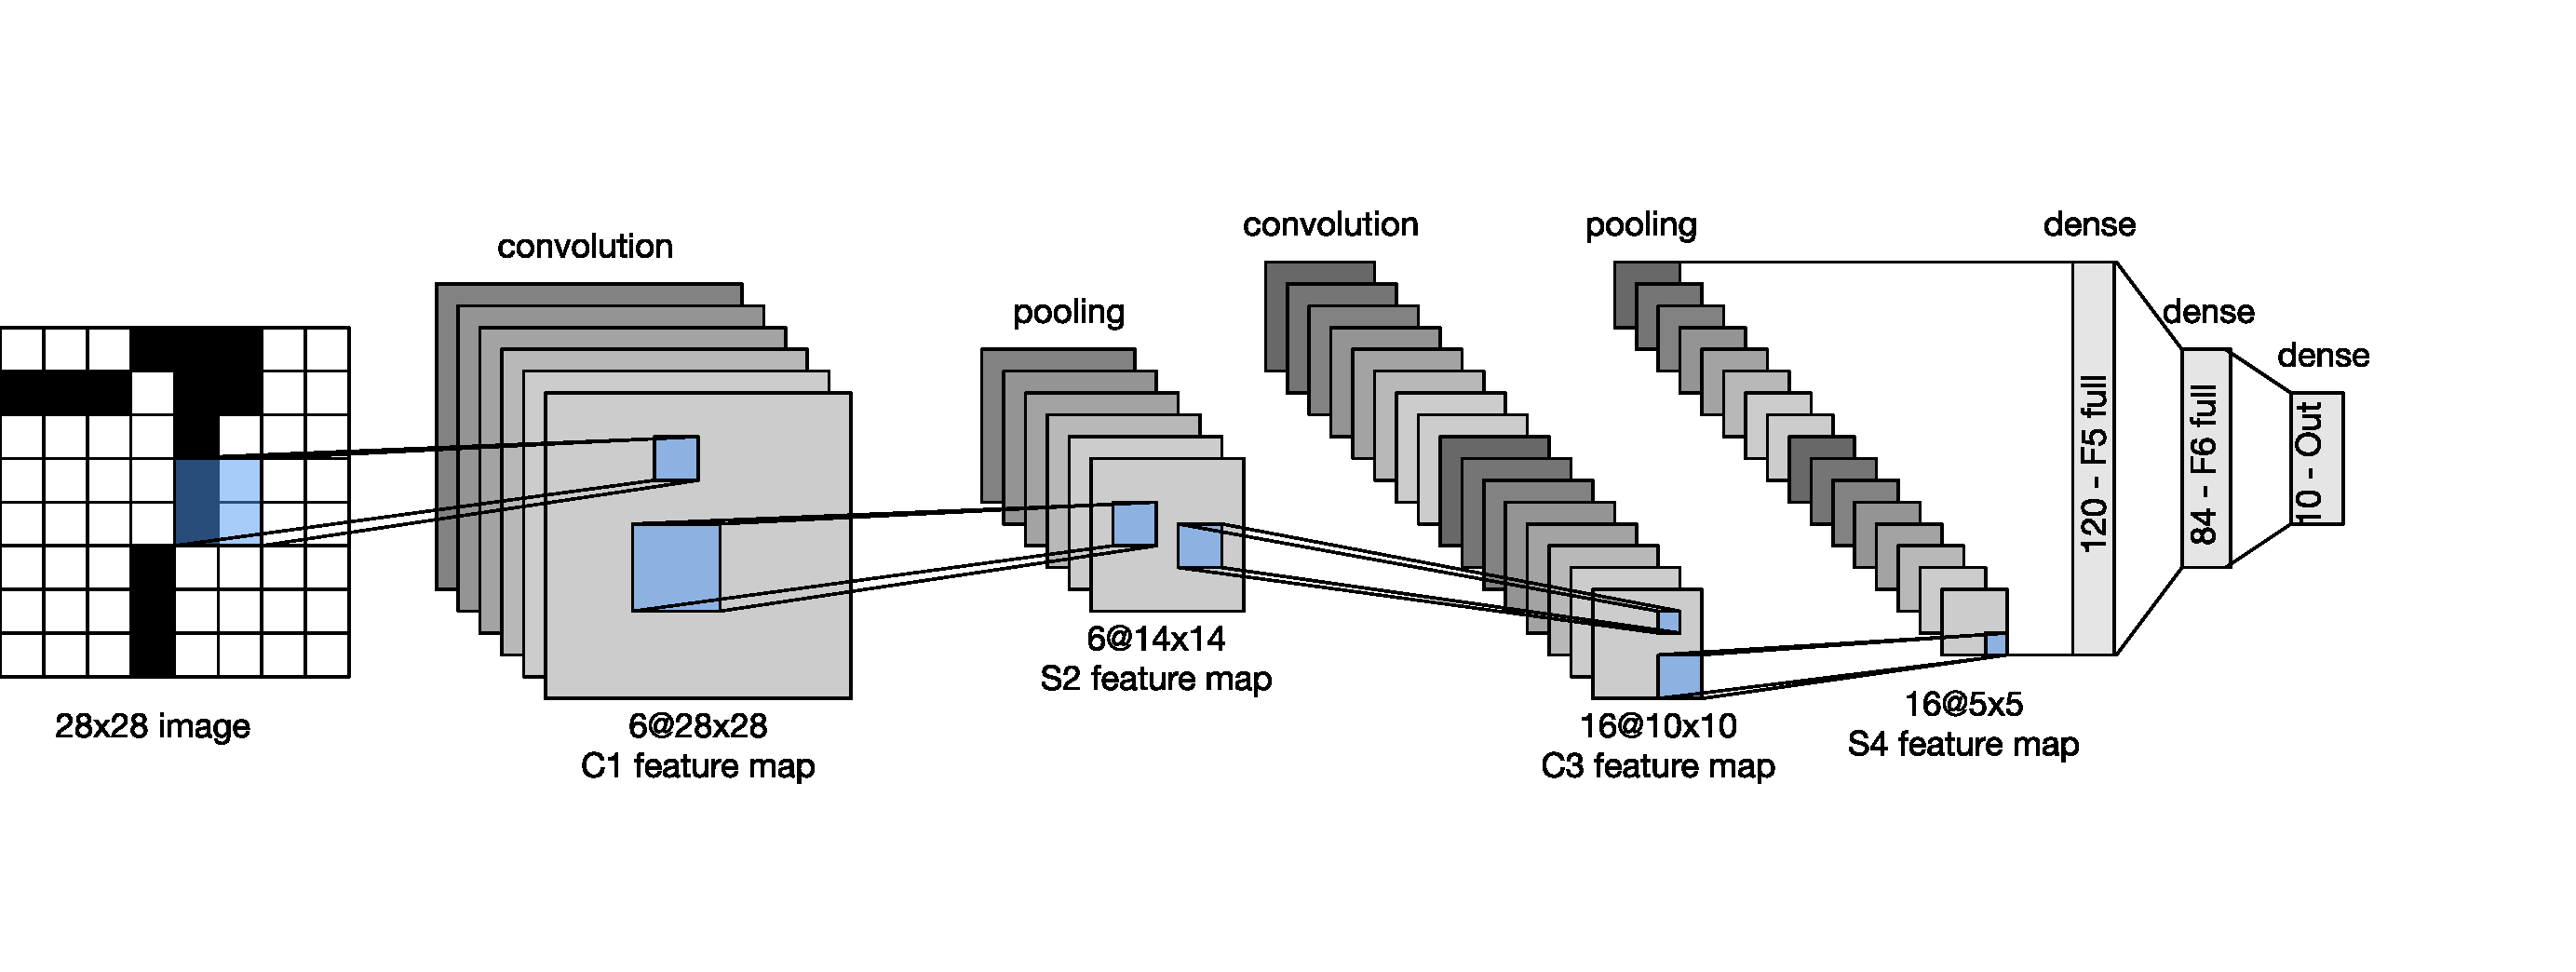
\includegraphics[width=150mm]{CNN}
  \caption[Convolutional Neural Network architecture]{Convolutional Neural Network architecture}
  \label{fig:cnn}
\end{figure}

\subsection{Generative models}

In machine learning, there are mainly three types of learning algorithms: supervised learning algorithms, unsupervised learning algorithms, and semi-supervised learning algorithms. The supervised learning algorithms are the type of algorithms that make use of labeled data for its training process. In the last years, this kind of algorithm is presenting very important results in applications like object detection \cite{Liu2019}.

The unsupervised learning algorithms are the ones that do not need a structured dataset and can find a pattern by itself. One particular type of unsupervised learning algorithms are the generative models. The generative models are powerful algorithms that are capable of learning the probabilistic data distribution of some datasets, allowing them to generate new samples. Two of the most important generative models are the variational autoencoders (VAE) and the generative adversarial networks (GAN).

\subsubsection{Autoencoders}

In a similar way as the CNNs, the autoencoders are an extension of the deep feedforward network, with the difference that in this case, the goal is to replicate the input in the output. This type of networks are divided into two parts: the encoder that tries to generate a latent space \begin{math}h\end{math} where is extracted some features of the input data \begin{math} h = f(x) \end{math}; and the decoder that takes the latent space generated by the encoder as input and reconstruct the data \begin{math} r = g(h) \end{math}. One of the main applications of the type of neural networks is the dimensionality reduction, image compression, image denoising or image generation. The image generation case shall be cover in more detail in the next section with the variational autoencoders as part of the generative models.

\begin{figure}[htb]
  \centering
  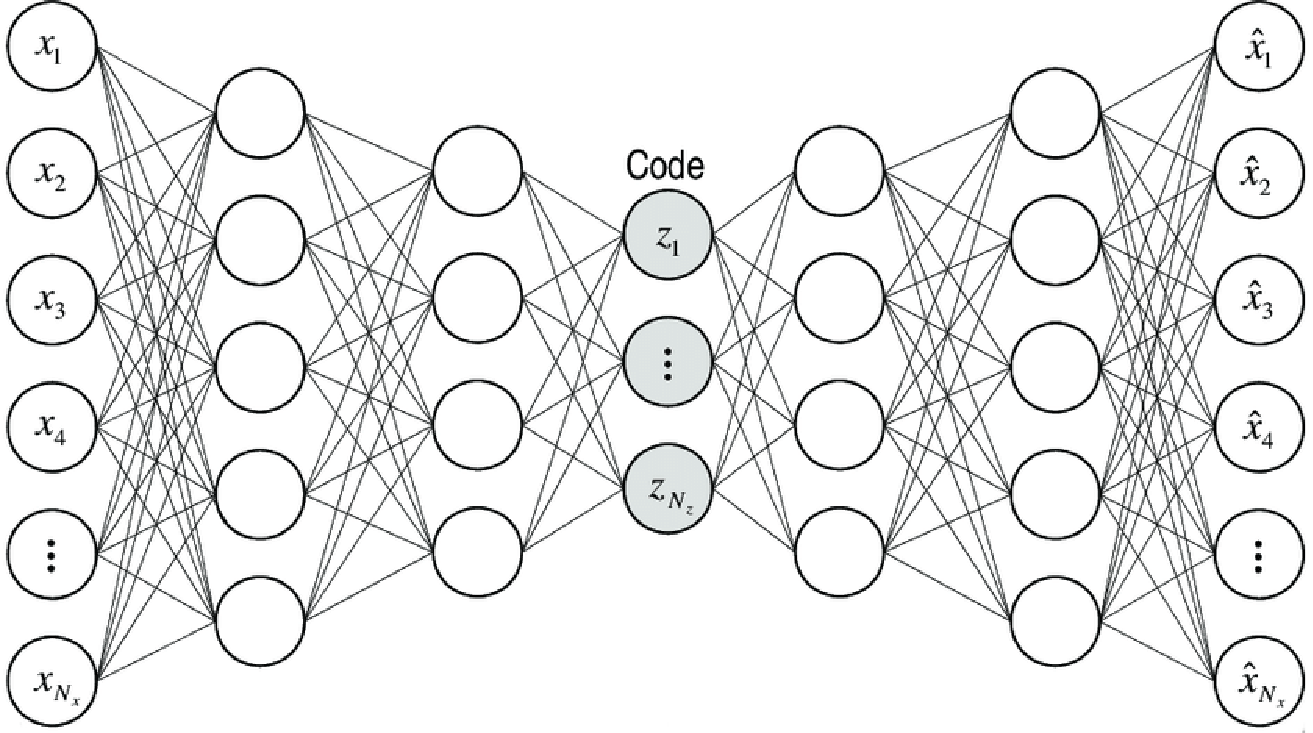
\includegraphics[width=80mm]{autoencoder}
  \caption[Autoencoder architecture]{Autoencoder architecture}
  \label{fig:autoencoder}
\end{figure}

\textit{Variational Autoencoder}

The objective of the variational autoencoders \cite{Kingma2014} is the generation of data samples from a learned latent space. This latent space is obtained from a large dataset. In order to achieve this generation process, this autoencoders must try to learn the probability distribution \begin{math} P(x) \end{math} of the data.

From a probabilistic perspective, the latent variables will be get from a prior \begin{math} P(z) \end{math} and the generated data has a likelihood of \begin{math} P(X|z) \end{math} that is conditioned by the latent space. So the goal here is to model de data distribution as follows:

\begin{equation}
 \mathbb{P}(\mathbf{X})=\int_{z} \mathbb{P}(\mathbf{X} | z) \mathbb{P}(z) d z
\end{equation}

However, this integral is computationally too costly, due to the fact of computing all the possibilities in the latent space. To avoid this, VAEs tries to infer the distribution \begin{math} \mathbb{P}( x ) \end{math} from data using \begin{math}\mathbb{P}(z|\mathbb{X})\end{math}. Variational inference approximates the distribution \begin{math}\mathbb{P}(z | \mathbb{X})\end{math}, using a simpler distribution, where a common choice is a Gaussian distribution. Then, with a parametric inference model \begin{math}\mathbb{Q}(z|\mathbb{X})\end{math} that maps the input data with the latent space; the difference between the distribution \begin{math}\mathbb{P}(z|\mathbb{X})\end{math} and \begin{math}\mathbb{Q}(z|\mathbb{X})\end{math} is calculated using the Kullback-Leibler divergence.

\begin{equation}
 \begin{aligned} D_{K L}(\mathbb{Q}(z | \mathbf{X}) \| \mathbb{P}(z | \mathbf{X})) &=\sum \mathbb{Q}(z | \mathbf{X}) \log \frac{\mathbb{Q}(z | \mathbf{X})}{\mathbb{P}(z | \mathbf{X})} \\ &=\mathbb{E}\left[\log \frac{\mathbb{Q}(z | \mathbf{X})}{\mathbb{P}(z | \mathbf{X})}\right] \\ &=\mathbb{E}[\log \mathbb{Q}(z | \mathbf{X})-\log \mathbb{P}(z | \mathbf{X})] \end{aligned}
 \label{eq:dkl}
\end{equation}

Using \begin{math}\mathbb{P}(z | \mathbf{X})=\frac{\mathbb{P}(\mathbf{X} | z) \mathbb{P}(z)}{\mathbb{P}(\mathbf{X})}\end{math}, the equation \ref{eq:dkl} can be rewritten as:

\begin{equation}
 \begin{aligned} D_{K L}(\mathbb{Q}(z | \mathbf{X}) \| \mathbb{P}(z | \mathbf{X})) &=\mathbb{E}\left[\log \mathbb{Q}(z | \mathbf{X})-\log \frac{\mathbb{P}(\mathbf{X} | z) \mathbb{P}(z)}{\mathbb{P}(\mathbf{X})}\right] \\ &=\mathbb{E}[\log \mathbb{Q}(z | \mathbf{X})-\log \mathbb{P}(\mathbf{X} | z)-\log \mathbb{P}(z)+\log \mathbb{P}(\mathbf{X})] \end{aligned}
\end{equation}

\begin{math}\mathbb{P}(x)\end{math} does not depend on \begin{math}z\end{math}, hence it can be taken out of the expectation:

\begin{equation}
 \begin{aligned} \Longrightarrow \log \mathbb{P}(\mathbf{X})-D_{KL}(\mathbb{Q}(z | \mathbf{X}) \| \mathbb{P}(z | \mathbf{X})) &=\mathbb{E}[\log \mathbb{P}(\mathbf{X} | z)]-\mathbb{E}[\log \mathbb{Q}(z | \mathbf{X})-\mathbb{P}(z)] \\ &=\mathbb{E}[\log \mathbb{P}(\mathbf{X} | z)]-D_{KL}(\mathbb{Q}(z | \mathbf{X}) \| \mathbb{P}(z)) \end{aligned}
\end{equation}

Therefore, the loss function corresponds to:

\begin{equation}
 \log \mathbb{P}(\mathbf{X}) \geq \mathbb{E}[\log \mathbb{P}(\mathbf{X} | z)]-D_{KL}(\mathbb{Q}(z | \mathbf{X}) \| \mathbb{P}(z))
\end{equation}

The first term of the loss function can be seen as the reconstruction error and the second term corresponds to the KL error \cite{Doersch2016}.

\textit{Spatial Variational Autoencoder}

Consist of an improvement of the typical variational autoencoder. Whereas in the classic VAEs the latent space are vectors where its variables have a dimension of 1x1, in the spatial VAE the idea is to extend these latent variables to have a bigger dimension and, in that way, be able to capture more spatial features of the input data.

In \cite{Wang2019} is proposes a spatial variational autoencoder, where the latent variables are sampled from a matrix-variable normal (MVN) distribution. The authors claim that this architecture outperforms the original VAEs due to the capture of richer structural and spatial information from data.

\textit{Gaussian-Mixure Variational Autoencoder}

This architecture corresponds to another variant of the VAEs models. In this case, the prior distribution \begin{math}\mathbb{P}(z)\end{math} is a Gaussian-mixture that allows the net to perform unsupervised clustering of the data. This autoencoder, proposed in \cite{Dilokthanakul2016}, has the potential of group the data, and each group can represent or share a specific feature of the original data, besides to have a competitive performance in comparison with the regular VAEs.

\subsubsection{Generative adversarial networks}

The generative adversarial networks (GAN) were proposed by Ian Goodfellow \cite{Goodfellow2014} in 2014. The basic idea behind GANs is in the competence of two models: from one side is the generator G that tries to learn the probability distribution of the data and for the other side, a discriminator \begin{math}\mathbb{D}\end{math} that decides if the input data is real or generated by \begin{math}\mathbb{G}\end{math}. The goal of the generator is to try to create images as real as possible that provokes the discriminator to make mistakes.  This game is described as the minmax value function in equation \ref{eq:gan}.

\begin{equation}
 \min _{G} \max _{D} V(D, G)=\mathbb{E}_{x \sim p_{\text {data }}(x)}[\log D(x)]+\mathbb{E}_{z \sim p_{z}(z)}[\log (1-D(G(z)))]
 \label{eq:gan}
\end{equation}

A well trained GAN model is able to reach the Nash equilibrium, where the discriminator has an accuracy of around 0.5, which means that it is not able to discern between fake or real data; and the generator should reach value loss of approximately 0.7.

\begin{figure}[htb]
  \centering
  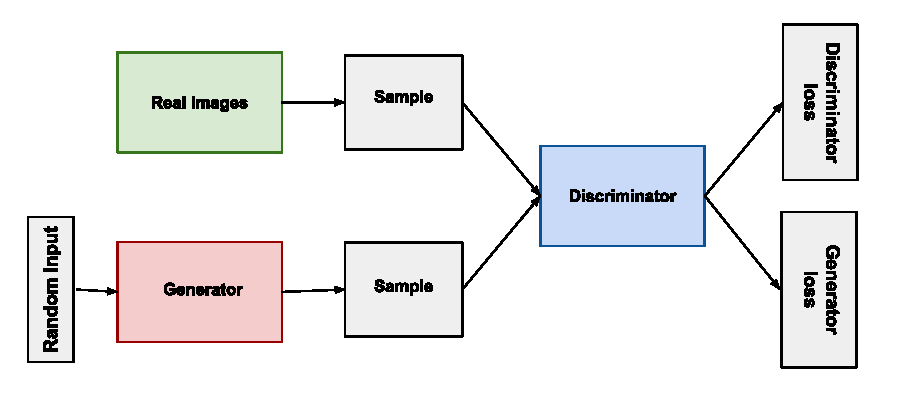
\includegraphics[width=120mm]{gan_diagram}
  \caption[Generative Adversarial Network architecture]{Generative Adversarial Network architecture}
  \label{fig:gan}
\end{figure}

One of the major challenges that the GANs has is precisely the training process, where sometimes is really hard to reach the Nash equilibrium. In some cases, if the capacity of the model is not enough, the model is susceptible to collapse. Another possible scenario is when the learning rate of the model is too aggressive, provoking that the net never converges.

\textit{Architectures based on GANs}

In \cite{Pan2019} presents a series of architectures based on GANs, along with some metrics to evaluate its performance.

\begin{itemize}
 \item \underline{Convolution base GAN}: The original GAN is implemented based on the multi-layer perceptron but it has been proven that CNN are better than the MLP in extracting features to the images. This kind of network is known as Deep Convolutional Generative Adversarial Network (DCGAN).
 \item \underline{Conditional GAN}: Normally, the generator of the GAN receives as input some random noise, which sometimes makes the model prone to collapse. It is for this reason that in the conditional GAN a variable C is introduced as input to the generator and also to the discriminator, with the objective of add some constraints and, therefore, have more control in that latent space. The type of constraint will depend on the type of data that the GAN is dealing with.
 \item \underline{Autoencoders based GANs}: This type of GAN architecture is presented in \cite{Makhzani2015} where the idea is to make use of an adversarial training to the autoencoder performing variational inference by matching the aggregated posterior latent space of the autoencoder with an arbitrary prior distribution. This will allow overcoming one of the main challenges of the autoencoders, where sometimes is not able to learn correctly the data distribution.
\end{itemize}

\subsection{Use of generative model in the anomaly detection}

The generative models discussed so far have their utility in the detection of anomalies. The general idea is to train a model to be able to learn the data distribution of a normal dataset. In that way, the model should be able to reconstruct o generate a query image as similar as possible. If for some reason that is not the case, there is a high probability that the regions that the model was not able to generate, correspond to an anomaly. All the autoencoders described before can be used in this way, as well as the GANs.

For the specific case of the GANs, in \cite{DiMattia2019} is presented different GAN based architectures, with the purpose of anomaly detection:

\subsubsection{AnoGAN}

This GAN is first trained with just normal data and be able to learn the manifold of the data X. Then, with the generator trained, each time that some image has to be evaluated, an iterative process is performed in order to find the latent variables that generate the more similar \begin{math}G(x)\end{math} to the query image. This iterative process has the disadvantage that is too time-consuming \cite{Schlegl2017}.

\begin{figure}[htb]
  \centering
  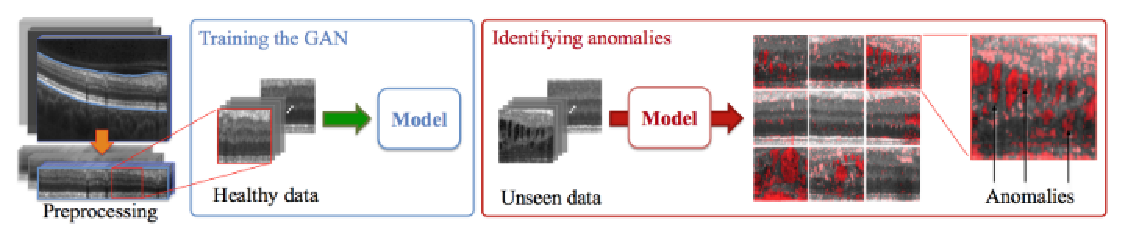
\includegraphics[width=150mm]{anogan}
  \caption[AnoGAN]{AnoGAN traing with healty images first and then reconstruction of unseen images\cite{Schlegl2017}}
  \label{fig:anogan}
\end{figure}

\subsubsection{GANomaly}

This architecture is inspired by the AnoGan but tries to overcome the long detection time that it has. In order to do that, make use of an encoder that is able to learn the latent space variables that the generator receives during the GAN training. This has the advantage of having a faster GAN training and reduces the times to generate a similar image to the query image. The generator also has an encoder at the end of its structure that helps in the training for the learning of the manifold of the input data \begin{math}x\end{math}.

\begin{figure}[htb]
  \centering
  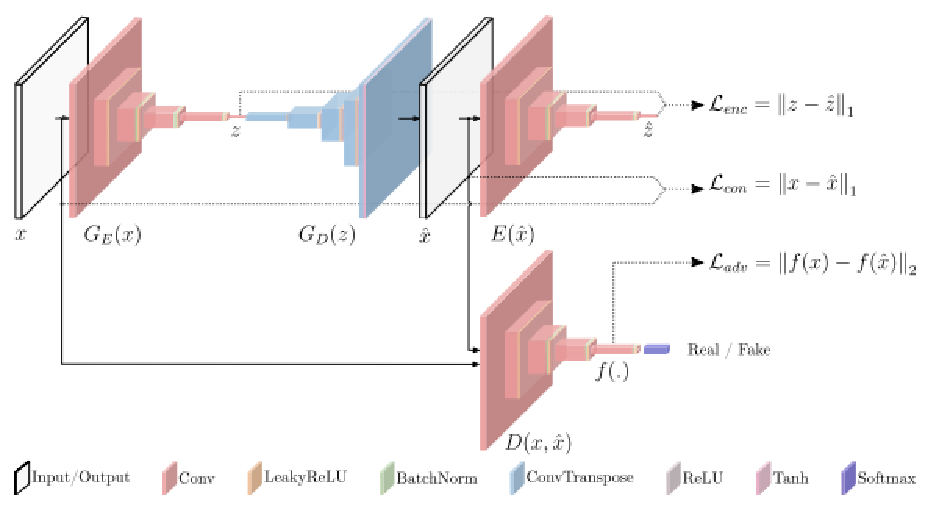
\includegraphics[width=130mm]{ganomaly}
  \caption[GANomaly]{GANomaly architecture and loss functions \cite{DiMattia2019}}
  \label{fig:ganomaly}
\end{figure}

  \chapter{Proposed solution}
\label{ch:solution}

\section{Data preprocessing}

The data acquired for this project used a camera of an iPhone 8 that captures in a resolution of 1920$\times$1080. The tomato data was captured in tomato crops located in the Alajuela province of Costa Rica (10$^{\circ}$01'39.2"N 84$^{\circ}$18'31.7"W). In the appendix \ref{ch:appendix} is described the capture protocole.

The comparison of anomaly detection models uses 191520 images with a size of 50$\times$50 each. For this set of images, 80\% was used for testing and 20\% used for validation. This training and validation data contains only healthy tomato plants. A set of 798 images is used for testing, and in this case, it also depicts unhealthy tomato plants.

Before using these images for training the models, a data normalization was applied to linearly map the image values to the range between -1 to 1. Additionally, image data augmentation as rotation, zoom, width shift, among other image transformations were implemented.

\section{Architecture experiment}

In order to evaluate the selected architectures for anomaly detection in tomato plants, an experiment of three architectures are proposed: one to explore the adversarial anomaly detector architecture, another to evaluate the spatial variational autoencoder and a third experiment to make use of the gaussian-mixture variational autoencoder.

All the architectures use the same dataset and for each one its reconstruction of an input image is tested by measuring the distance between the original and reconstructed images using the mean square error (MSE). The expected behavior here is that, as the model is only trained with healthy images of tomato, if some input image presents a possible disease, the model should not be able to reconstruct the affected area, and that reconstruction error or dissimilarity is an indication of the presence of an anomaly.

\section{Contribution}

The architecture proposed in this project is an adversarial anomaly detector inspired in the AnoGAN. This architecture is composed of the typical generator and discriminator of a GAN, but with the addition of an encoder \begin{math}E(x) = z\end{math} that is connected with the generator input.

The training process of this approach has two stages: First the the GAN is trained with the conventional methods, but exclusivelly using healthy images of tomato, where the generator receives random noise as input for the latent variables. The second stage is training the encoder that has to learn how to map the query input image into the latent space.

During training of the encoder, the generator and discriminator models remain unchanged. Also, the hidden layers of the discriminator are used to extract features of the synthetic images and the input images. The goal is to train the encoder in a way that it forces the generator to create images with similar features as the ones of the query image.

The proposed loss function for this anomaly detector model is the following:

\begin{equation}
 \mathcal{L}\left(\mathbf{E}(x)\right)=(1-\lambda) \cdot \mathcal{L}_{R}\left(\mathbf{E}(x)\right)+\lambda \cdot \mathcal{L}_{D}\left(\mathbf{E}(x)\right)
\end{equation}

where \begin{math}\lambda\end{math} weights both terms of the function and $\mathbf{E}$ is the Encoder. \begin{math}\mathcal{L}_{R}\end{math} (reconstruction error) and \begin{math}\mathcal{L}_{D}\end{math} (discriminator error) are defined as:

\begin{equation}
 \mathcal{L}_{R}\left(\mathbf{E}(x)\right)=\left\|\mathbf{x}-G\left(\mathbf{E}(x)\right)\right\|
\end{equation}

\begin{equation}
 \mathcal{L}_{D}\left(\mathbf{E}(x)\right)=\left\|\mathbf{f}(\mathbf{x})-\mathbf{f}\left(G\left(\mathbf{E}(x)\right)\right)\right\|
\end{equation}

where \begin{math}\mathbf{f}(x)\end{math} represents the feature extractor of the discriminator.

This approach overcomes one of the disadvantages of the AnoGAN that is its long computational time. This modification of the AnoGAN architecture is similar to the one presented in \cite{Schlegl2019}.

  \chapter{Results and analysis}
\label{ch:results}

From a qualitative evaluation of the three architectures: Adversarial Anomaly Detector, sVAE, and GM-VAE; the one presenting the best reconstruction is the Adversarial Anomaly Detector. For the two autoencoders, the reconstructions suffer from blurring (see figures \ref{fig:svae_rec} and \ref{fig:gmvae_rec}), making it difficult to evaluate the presence of an anomaly and hence confirming one of the main problems of this kind of autoencoders. The problems in the autoencoders could the caused for the bias the learned data distribution has, due to the simpler data distributions underlying the model.

\begin{figure}[H]
\begin{minipage}{\linewidth}
  \centering
  \begin{tabular}{ccc}
  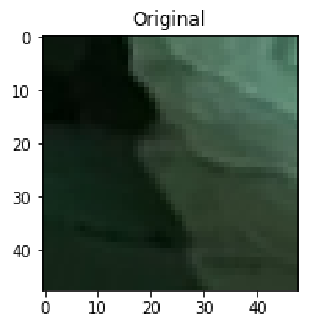
\includegraphics[width=.25\linewidth]{anogan_sample1_original}
    & 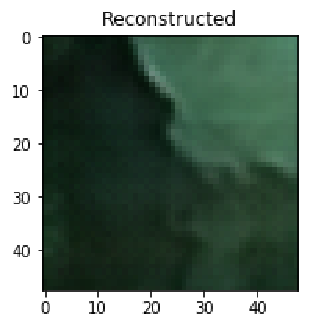
\includegraphics[width=.25\linewidth]{anogan_sample1_reconstruction} \\
  (a) & (b) \\
  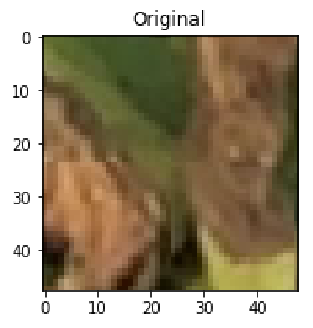
\includegraphics[width=.25\linewidth]{anogan_sample2_original}
    & 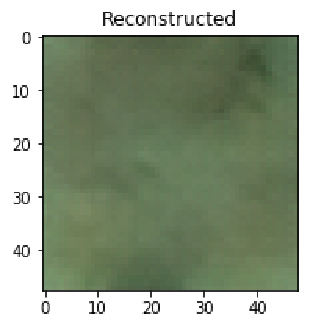
\includegraphics[width=.25\linewidth]{anogan_sample2_reconstruction} \\
  (c) & (d)
  \end{tabular}
  \end{minipage}
\caption[Reconstruction example of the adversarial anomaly detector]{Reconstruction example of the adversarial anomaly detector: a) origianl healthy sample, b) reconstructed healthy sample, c) original test sample and d) reconstructed test sample.}
\label{fig:anogan_rec}
\end{figure}

\begin{figure}[H]
\begin{minipage}{\linewidth}
  \centering
  \begin{tabular}{ccc}
  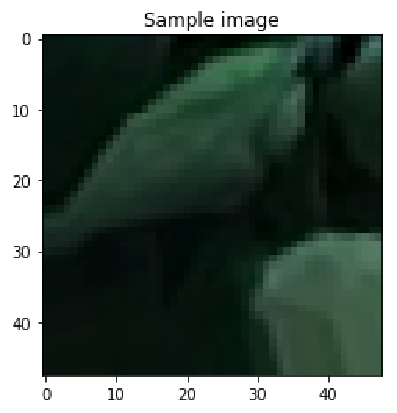
\includegraphics[width=.25\linewidth]{svae_sample1_original}
    & 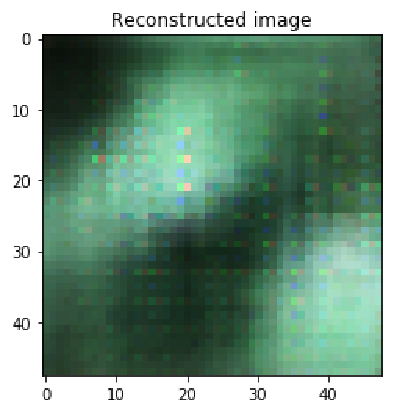
\includegraphics[width=.25\linewidth]{svae_sample1_reconstruction} \\
  (a) & (b) \\
  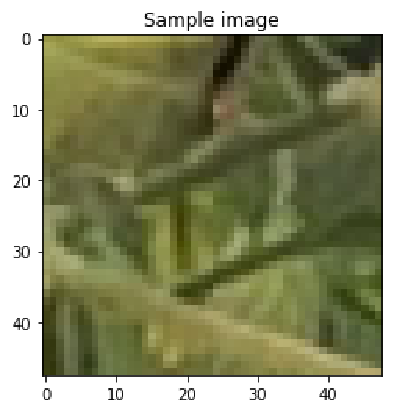
\includegraphics[width=.25\linewidth]{svae_sample2_original}
    & 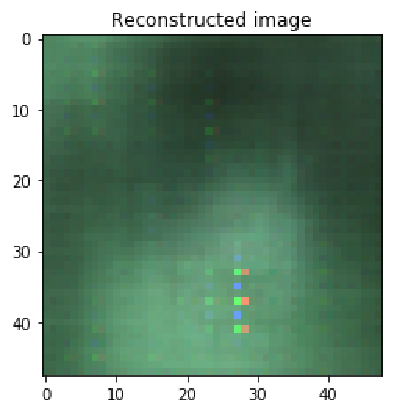
\includegraphics[width=.25\linewidth]{svae_sample2_reconstruction} \\
  (c) & (d)
  \end{tabular}
  \end{minipage}
\caption[Reconstruction example of the sVAE]{Reconstruction example of the sVAE: a) original healthy sample, b) reconstructed healthy sample, c) original test sample and d) reconstructed test sample.}
\label{fig:svae_rec}
\end{figure}

\begin{figure}[H]
\begin{minipage}{\linewidth}
  \centering
  \begin{tabular}{ccc}
  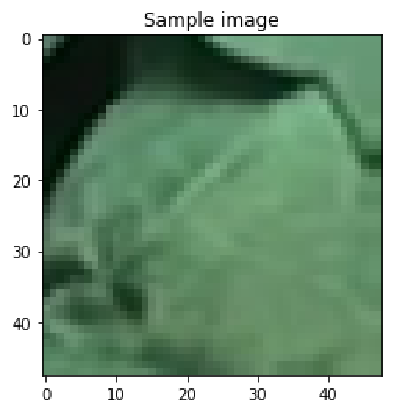
\includegraphics[width=.25\linewidth]{gmvae_sample1_original}
    & 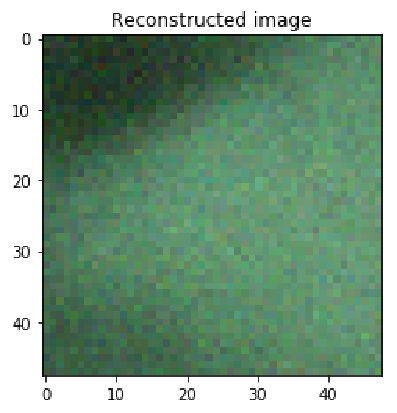
\includegraphics[width=.25\linewidth]{gmvae_sample1_reconstruction} \\
  (a) & (b) \\
  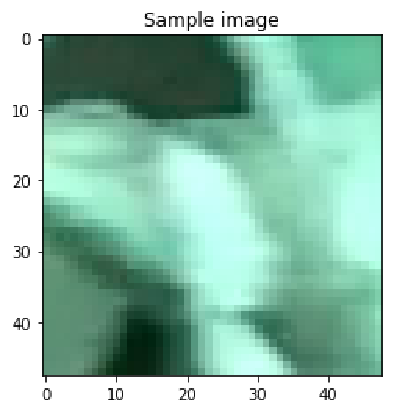
\includegraphics[width=.26\linewidth]{gmvae_sample2_original}
    & 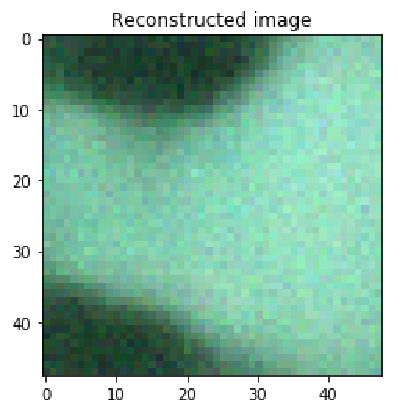
\includegraphics[width=.25\linewidth]{gmvae_sample2_reconstruction} \\
  (c) & (d)
  \end{tabular}
  \end{minipage}
\caption[Reconstruction example of the GM-VAE]{Reconstruction example of the GM-VAE: a) original healthy sample, b) reconstructed healthy sample, c) original test sample and d) reconstructed test sample.}
\label{fig:gmvae_rec}
\end{figure}

\begin{figure}[htb]
  \centering
  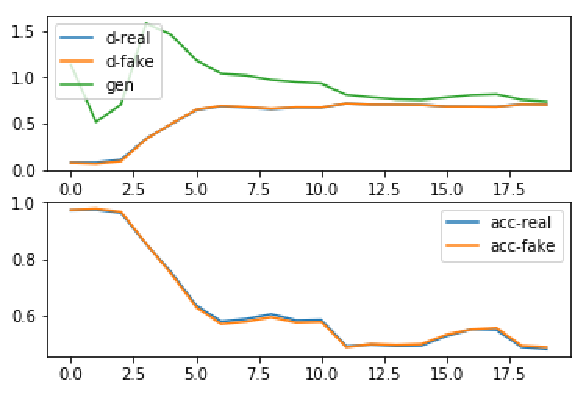
\includegraphics[width=100mm]{gan_training}
  \caption[GAN training]{GAN training: the top graph shows the loss of the generator and the discriminator. The bottom graph shows the accuracy of the discriminator for real and fake images. }
  \label{fig:gan_training}
\end{figure}

The group of healthy samples are extracted from figure \ref{fig:test_images}.a and for the anomalies samples are extracted from figure \ref{fig:test_images}.b. In the case of the AnoGAN, the training of the model is unstable, but with the available tomato data, it was possible to achieve the Nash equilibrium (see figure \ref{fig:gan_training}). The generated images are better than the ones in the autoencoders as can be seen in table \ref{table:rec_eval} with the values of mean and standard deviation (STD) of the healthy and anomaly samples. Its main disadvantage is the time needed to learn a set of latent variables to reconstruct some images. This problem is resolve with the introduction of an encoder in the AnoGAN architecture as shown in the table \ref{table:rec_time} where the reconstruction times are shown for the different models.

\begin{table}[htb]
    \caption[Reconstruction time evaluation]{Reconstruction time evaluation.}
    \label{table:rec_time}
    \centering
    \begin{tabular}{ c c c }
        \hline
        Model & Reconstruction time (ms) \\
        \hline
        sVAE & 160.8 \\
        GM-VAE & 1383.1 \\
        AnoGAN & 6320.6 \\
        Adversarial Anomaly Detector & 255.3 \\
        \hline
    \end{tabular}
\end{table}

Figure \ref{fig:rec_eval} has the reconstruction scores distribution of regular and anomalous samples for the three models. This figure also shows that the best model for the reconstruction of regular samples is the Adversarial Anomaly detector, however, there are still some samples that are indiscernible between regular or anomalous. For that reason explore more metrics would be needed.

\begin{table}[htb]
    \caption[Reconstruction metric evaluation]{Reconstruction metric evaluation.}
    \label{table:rec_eval}
    \centering
    \begin{tabular}{ c c c c c }
        \hline
        Model & Mean (healthy) & STD (healthy) & Mean (anomalies) & STD (anomalies) \\
        \hline
        sVAE & 10410.6 & 7020.3 & 19858.8 & 18464.1 \\
        GM-VAE & 15162.2 & 7597.3 & 9357.3 & 6071.7 \\
        AAD & 3839.5 & 3251.1 & 8996.1 & 3308.8 \\
        \hline
    \end{tabular}
\end{table}

\begin{figure}[H]
\begin{minipage}{\linewidth}
  \centering
  \begin{tabular}{ccc}
  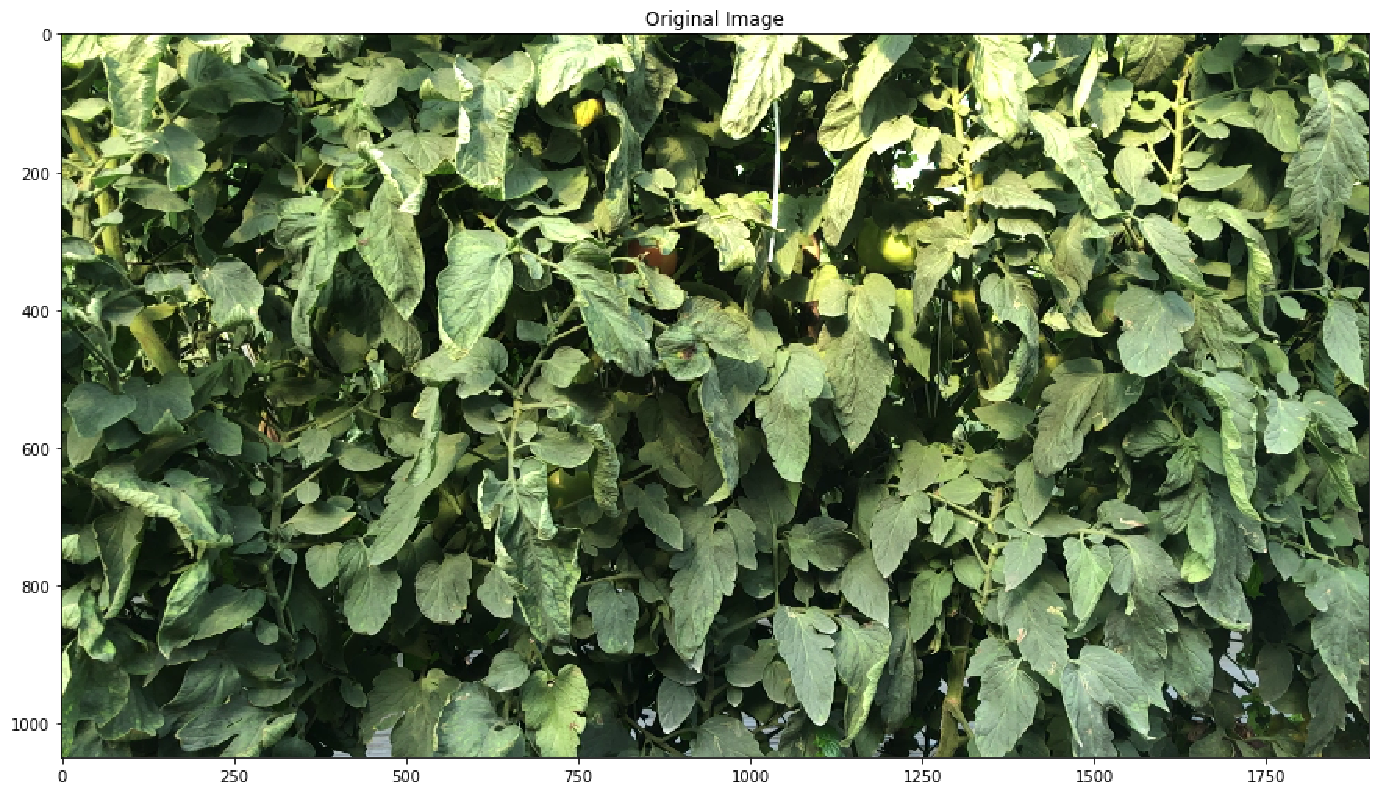
\includegraphics[width=125mm]{anogan_test_image1} \\
  (a) \\ 
  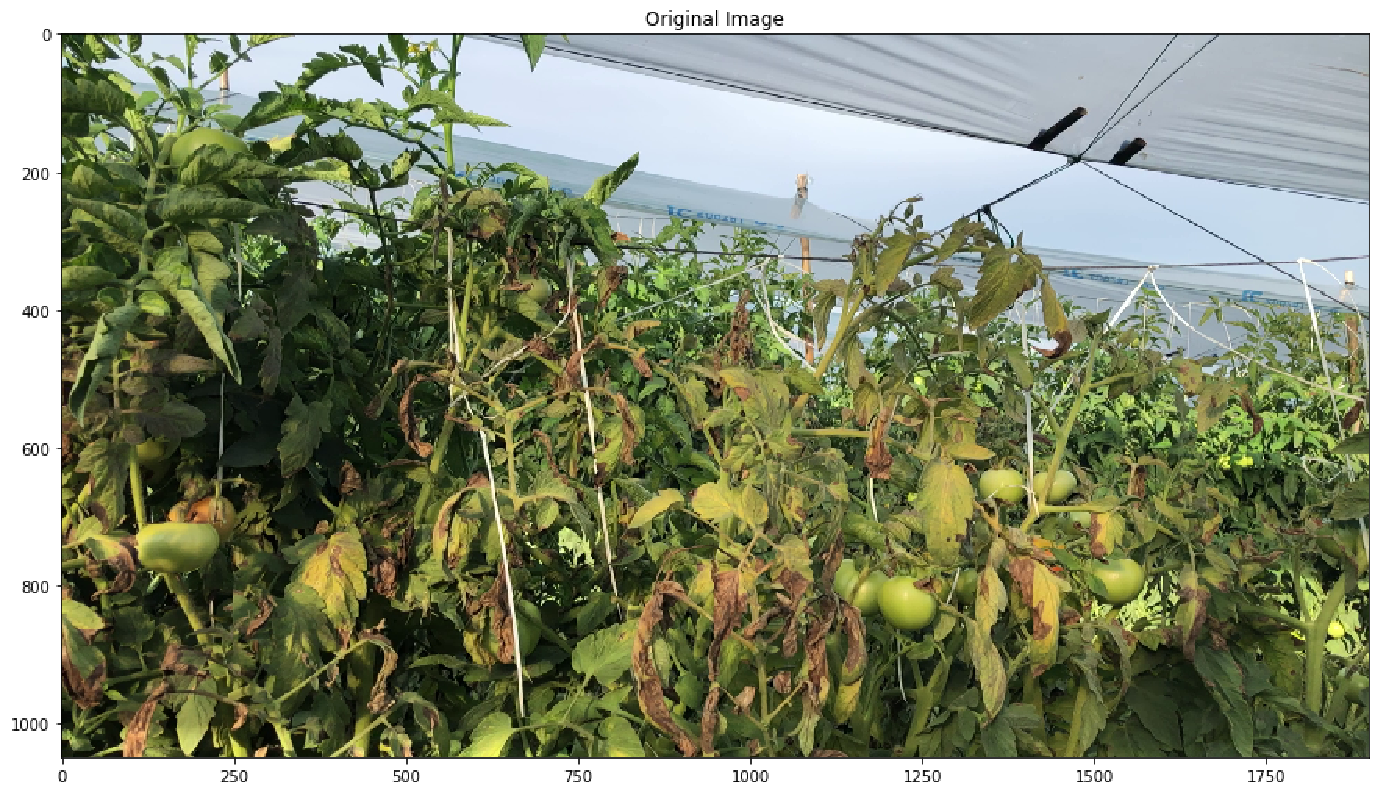
\includegraphics[width=125mm]{anogan_test_image2} \\
  (b) \\
  \end{tabular}
  \end{minipage}
\caption[Experiment test images]{Experiment test images: a) healthy image and b) anomlous image.}
\label{fig:test_images}
\end{figure}

In figures \ref{fig:anogan_eval_test_image_1} and \ref{fig:anogan_eval_test_image_2} depict the data distribution between regualr and anomalous samples. Figure \ref{fig:anogan_eval_test_image_1} shows a defined group of data that represents the healthy samples and a smaller amount of points around this healthy group that represents anomalous data. In figure \ref{fig:anogan_eval_test_image_2} we have the opposite case, where the number of anomalies is larger than the number of healthy samples. For the first case, the test images depict a tomato plant in a healthy state, and for the second case, the tomato plant presented several affections, fact that is reflected in each of the graphs mentioned before.

\begin{figure}[h]
\begin{minipage}{\linewidth}
  \centering
  \begin{tabular}{ccc}
  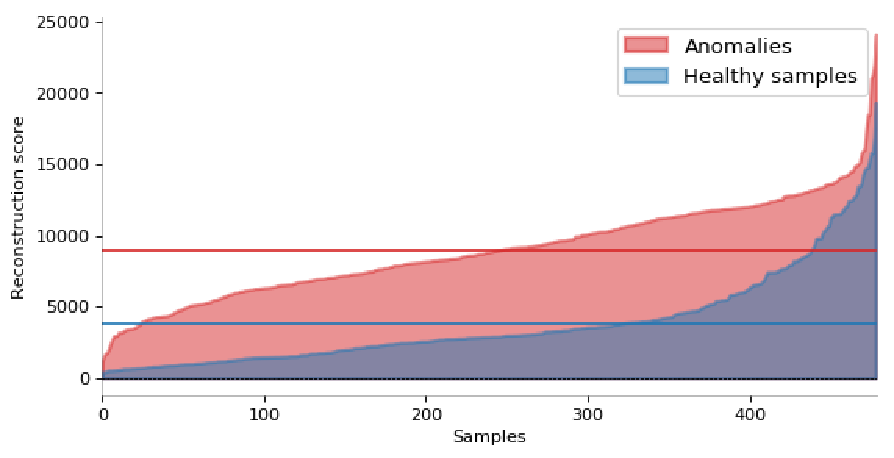
\includegraphics[width=120mm]{rec_anogan_eval} \\
  (a) \\ 
  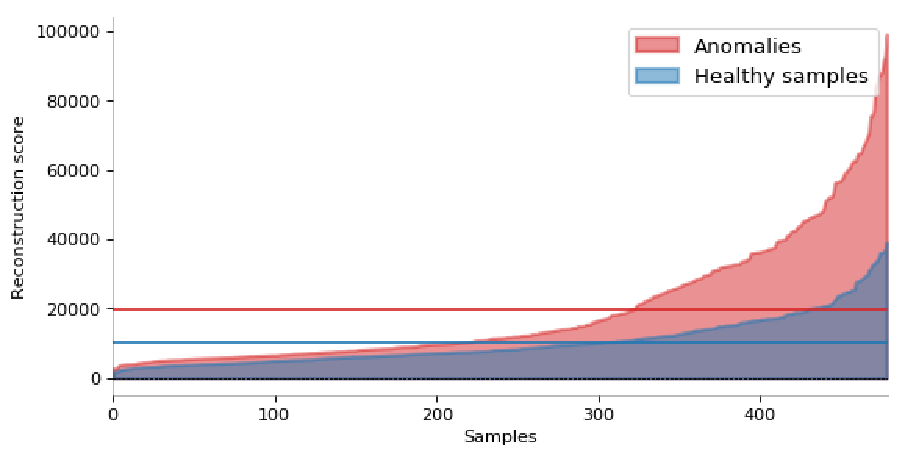
\includegraphics[width=120mm]{rec_svae_eval} \\
  (b) \\ 
  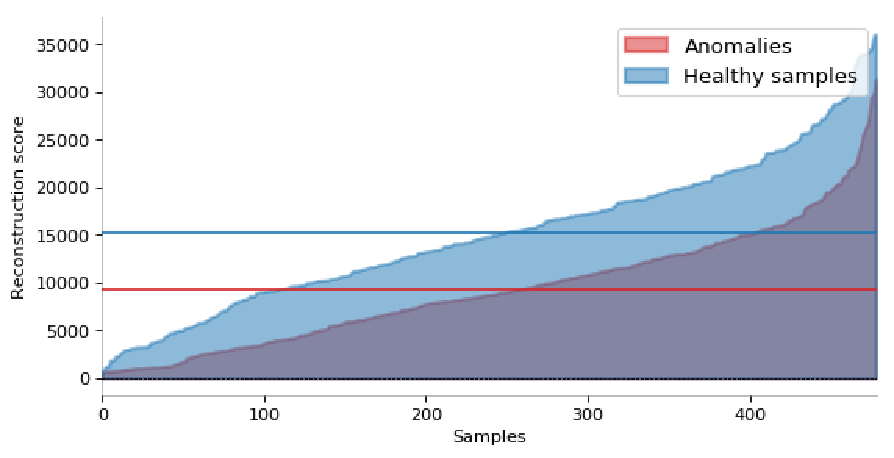
\includegraphics[width=120mm]{rec_gmvae_eval}\\
  (c) \\
  \end{tabular}
  \end{minipage}
\caption[Reconstruction evaluation of the Adversarial Anomaly Detectof, sVAE and GM-VAE]{Reconstruction evaluation of the a) Adversarial Anomaly Detectof, b) sVAE and c) GM-VAE. The horizontal lines represents the mean value of the healty samples and the anomaly samples.}
\label{fig:rec_eval}
\end{figure}

\begin{figure}[htb]
  \centering
  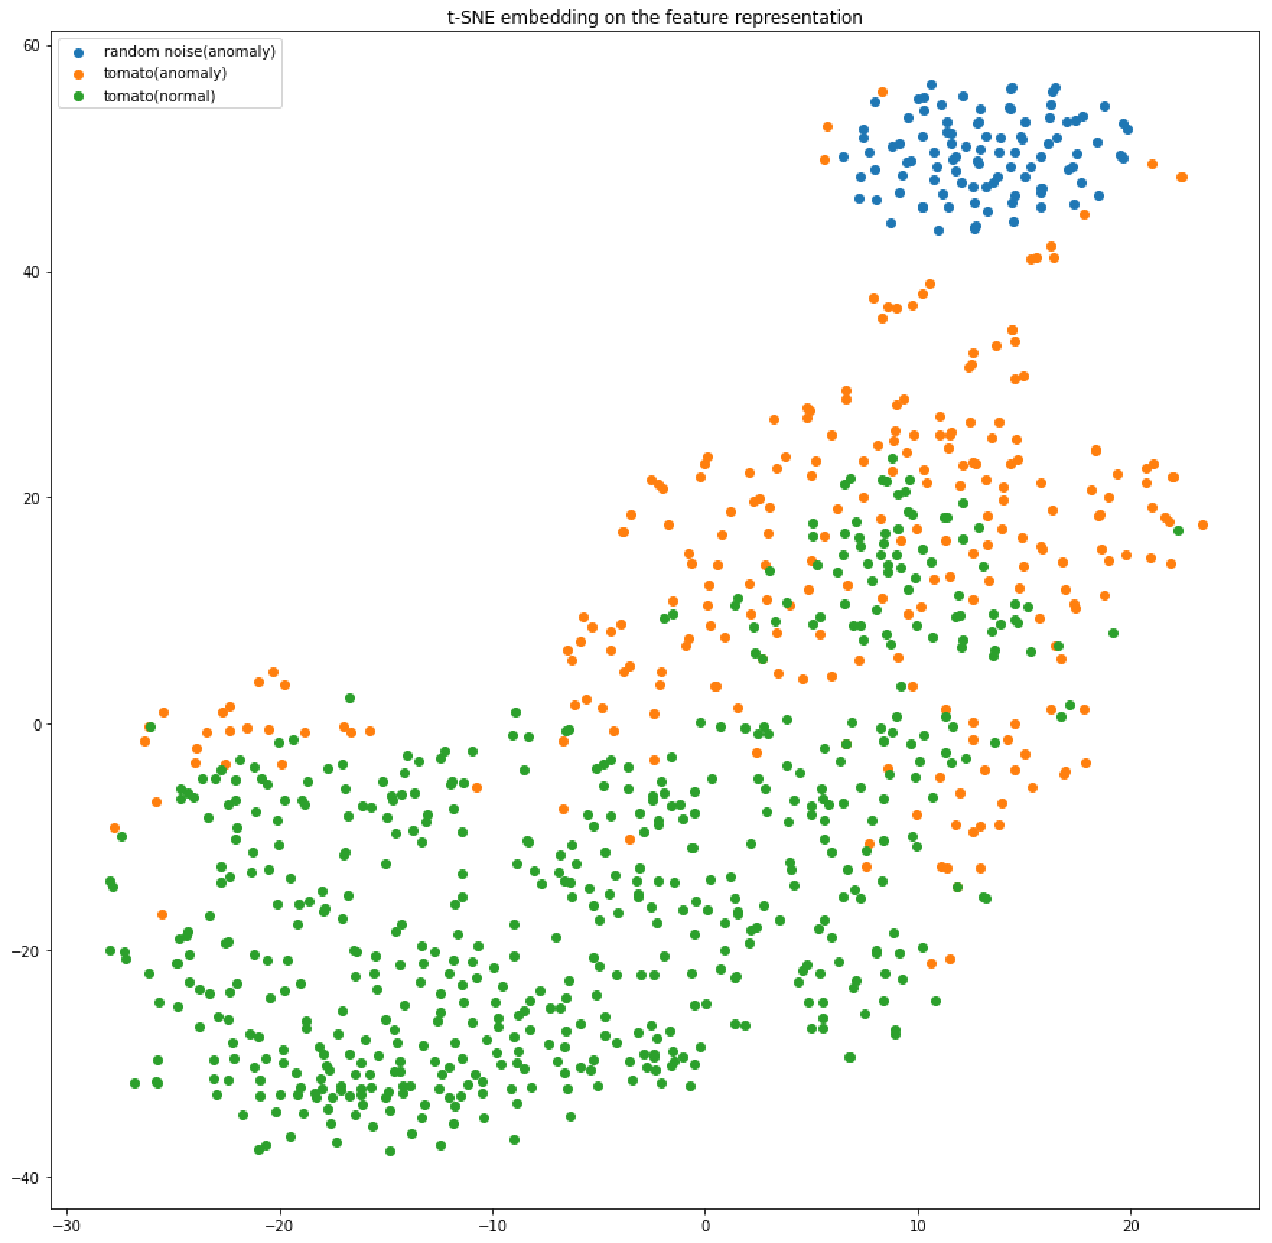
\includegraphics[width=150mm]{anogan_t_sne1}
  \caption[Adversarial Anomaly Detector t-SNE evaluation of test image 1]{Adversarial Anomaly Detector t-SNE evaluation of test image 1}
  \label{fig:anogan_eval_test_image_1}
\end{figure}

\begin{figure}[htb]
  \centering
  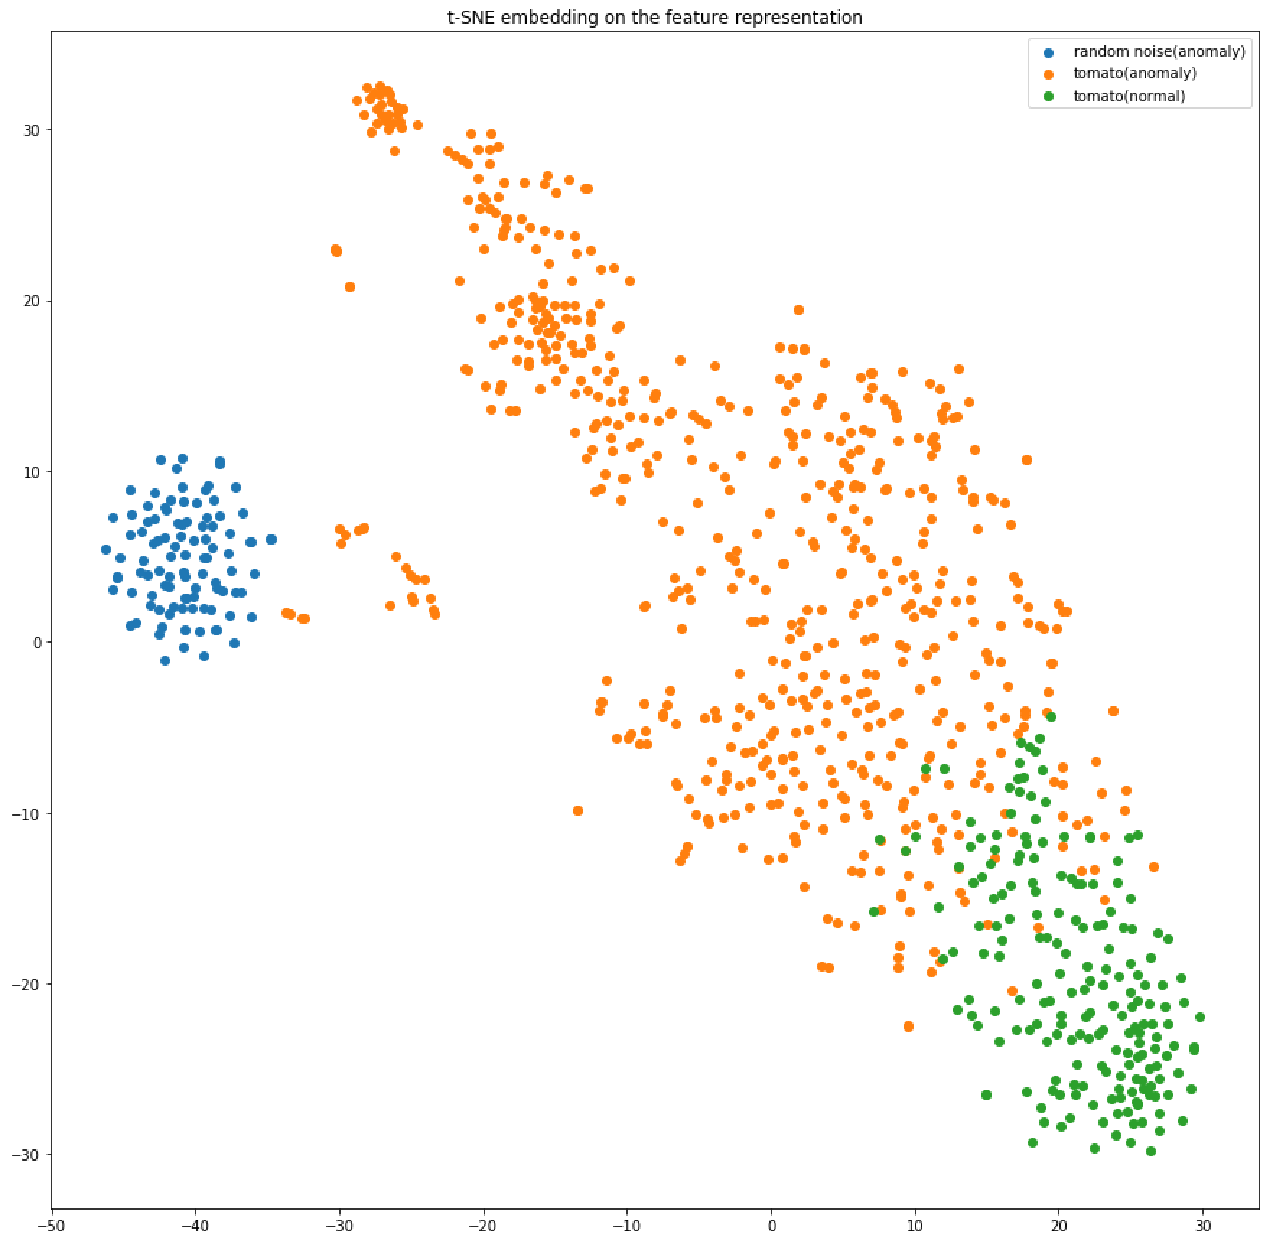
\includegraphics[width=150mm]{anogan_t_sne2}
  \caption[Adversarial Anomaly Detector t-SNE evaluation of test image 2]{Adversarial Anomaly Detector t-SNE evaluation of test image 2}
  \label{fig:anogan_eval_test_image_2}
\end{figure}

  \chapter{Conclusions}
\label{ch:conclusions}


  %----------------------------------------------------------------------------
  % literature in bibtex way:
  % \bibliographystyle{sty/plainurl} % for english documents
  % \bibliography{literatura}
  % literature in biblatex/biber way
  \printbibliography[title={Bibliography},heading=bibintoc]
  %----------------------------------------------------------------------------

  %----------------------------------------------------------------------------
  \appendix
  %----------------------------------------------------------------------------

  \chapter{Capture protocol}

The following document describes the capture protocol proposed for the thesis project Adversarial Anomaly Detector, which aims to be a guide to be followed by potential collaborators. It is important that the collaborator follow this guide in order to have the best data quality for the project.

\section{General considerations}

The data will be captured in the tomato crop field. Typically these plantations are divided into a large number of grooves, so it is intended to create videos that cover each of these grooves. The distance between the groove ranges from 1.8 to 2 meters. Figure [FIGURE] shows an example of a tomato plantation.

\begin{figure}[htb]
  \centering
  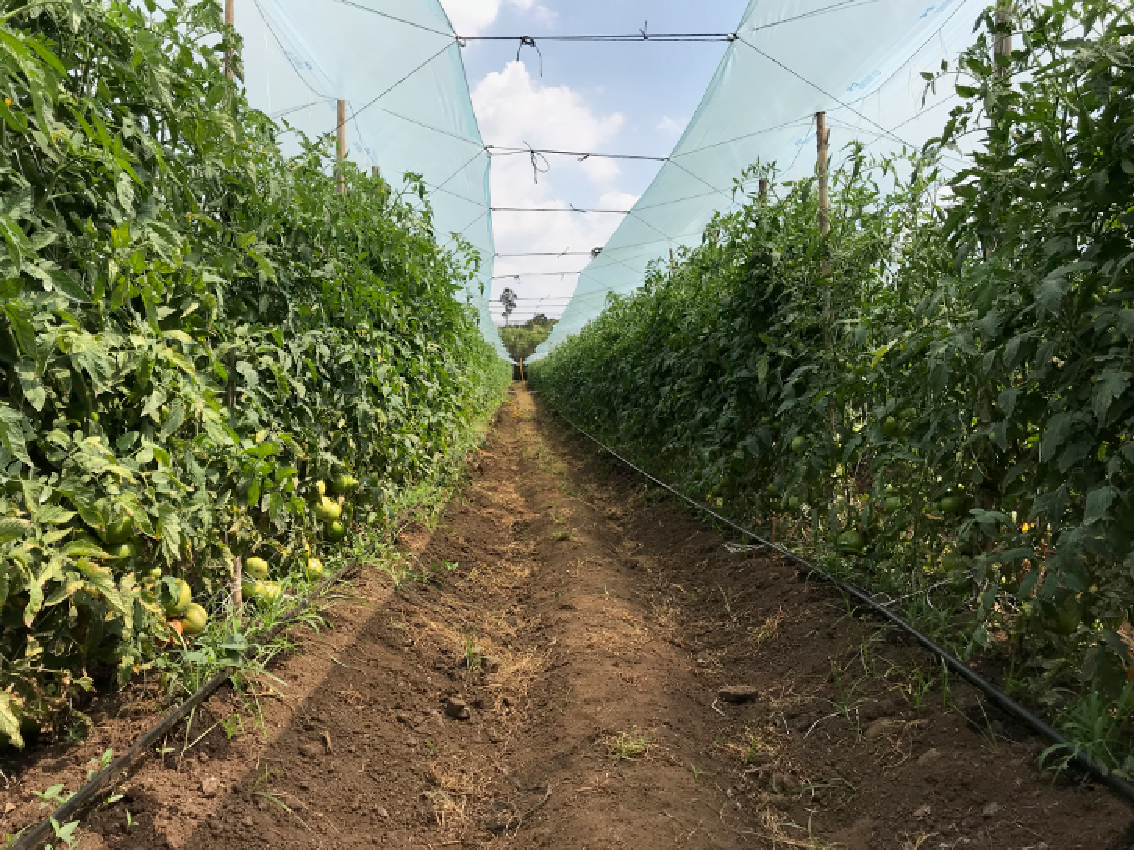
\includegraphics[width=100mm]{tomato_crop}
  \caption[Tomato crop]{Tomato crop in Costa Rica.}
  \label{fig:tomato_crop}
\end{figure}

\section{Video considerations}

\begin{itemize}
 \item The video resolution must be 1920x1080 pixels.
 \item Make use of a video stabilizer like a Gimbal. (For example the DJI Osmo Mobile 2)
 \item The video must be recorded in color.
 \item The duration of the video will depend on the length of the groove.
 \item The distance of the chamber from the plants should be approximately 1.5 meters.
 \item The video should cover the entire structure of the plant, from its base to the highest branches. If it is not possible to cover the entire plant in the same video, it will be done in different videos, covering in one of them the upper part of the plant and in another the lower part.
 \item Use the camera of a cell phone with Android or iOS operating systems.
 \item Use a mobile application that is capable of controlling the cell phone's front camera. Suggested applications: Filmic Pro.
 \item Utilizar una tarjeta de calibración de color previo a realizar los videos.
\end{itemize}

\section{Instructions for capturing the video}

As mentioned earlier, the videos cover each groove that confirms tomato plantations. Below are instructions to correctly capture the videos:

\begin{figure}[htb]
  \centering
  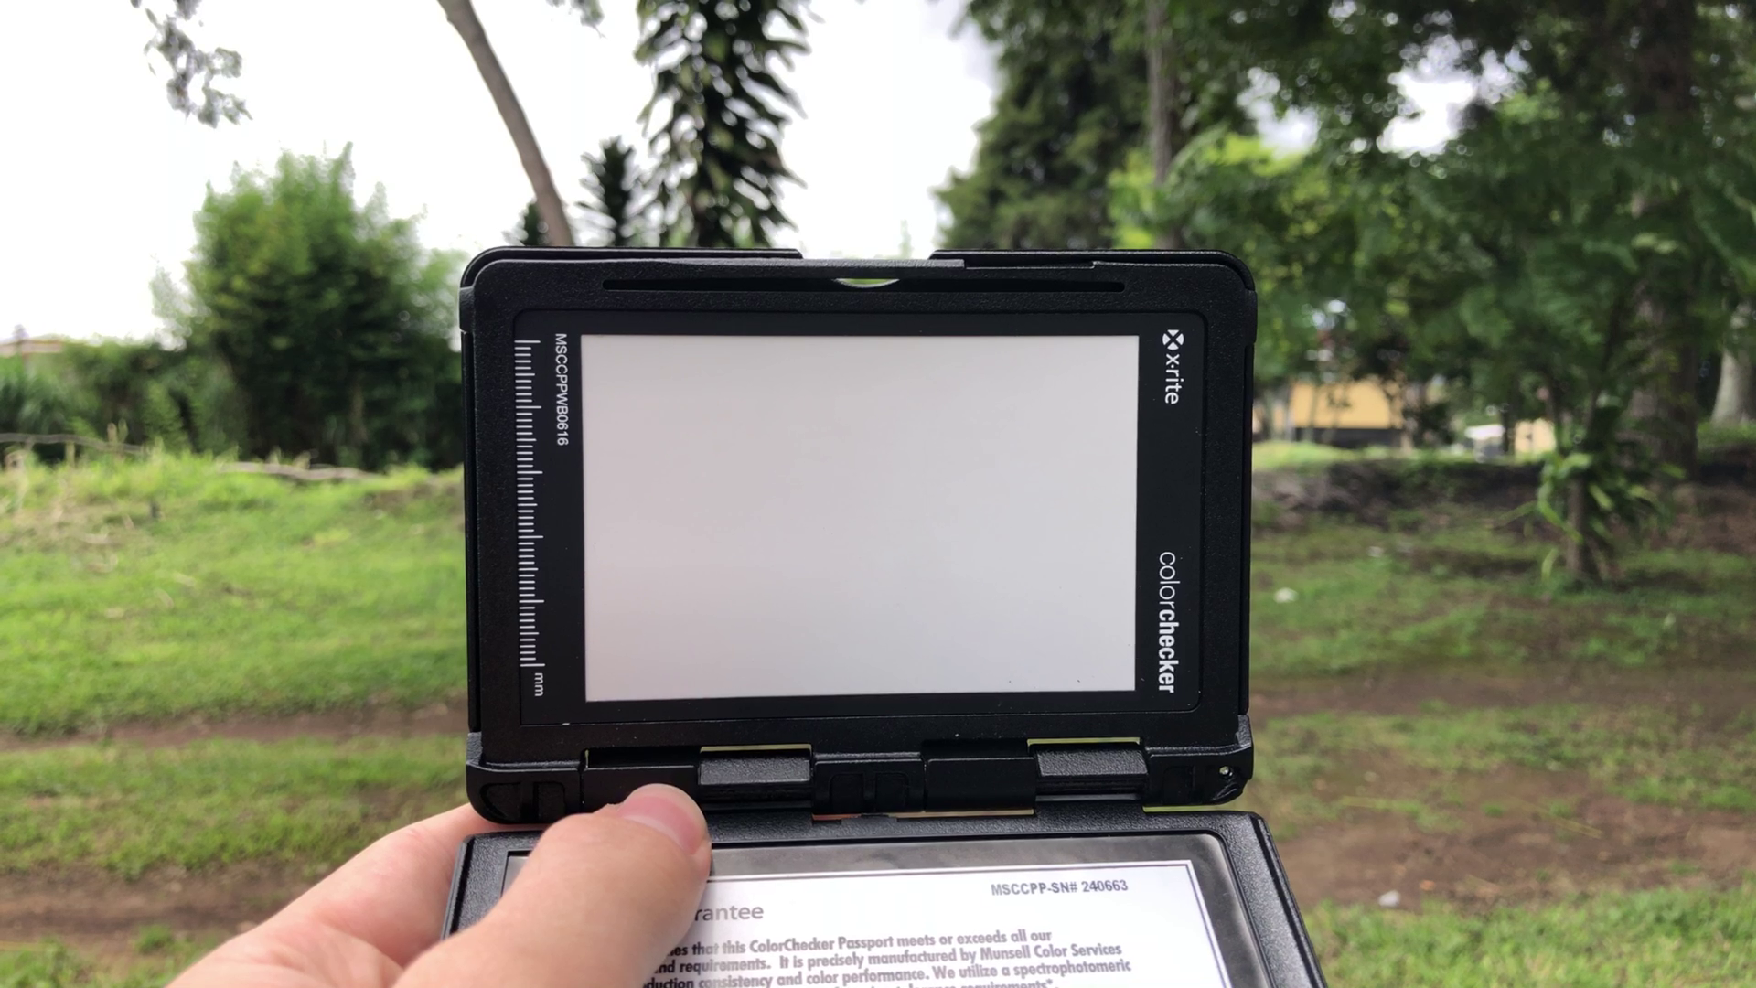
\includegraphics[width=100mm]{protocol2}
  \caption[Color calibration]{Colo checker gray card.}
  \label{fig:color_calibration}
\end{figure}

\subsection{Color calibration}

Using a gray scale calibration card, the camera's white balance should be adjusted as follows.

\begin{enumerate}
 \item Enter to the Filmic Pro application.
 \item Position the calibration card in front of the camera and zoom in to focus on the card only.
 \item Go to the camera settings and select the section related to white balance.
 \item Select the option to perform an automatic white balance.
 \item Wait a moment for the camera's white balance to be automatically adjusted and then select the option to set the white balance.
 \item It is important to mention that this process must be carried out in the place where the capture is intended and it is also recommended to repeat the steps every 30 minutes, to anticipate possible changes in the lighting that the place presents.
\end{enumerate}

\begin{figure}[H]
\begin{minipage}{\linewidth}
  \centering
  \begin{tabular}{ccc}
  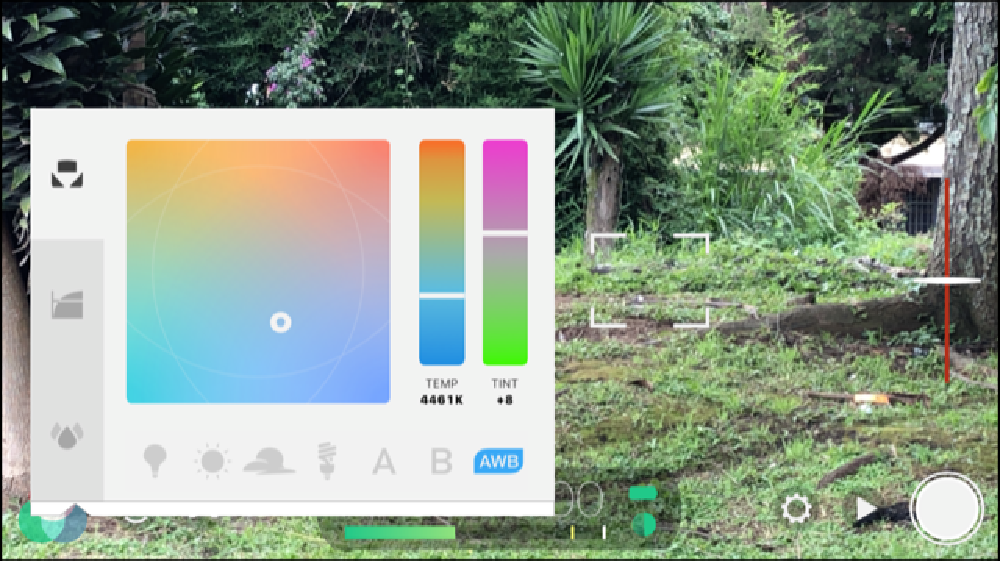
\includegraphics[width=.40\linewidth]{protocol4}
    & 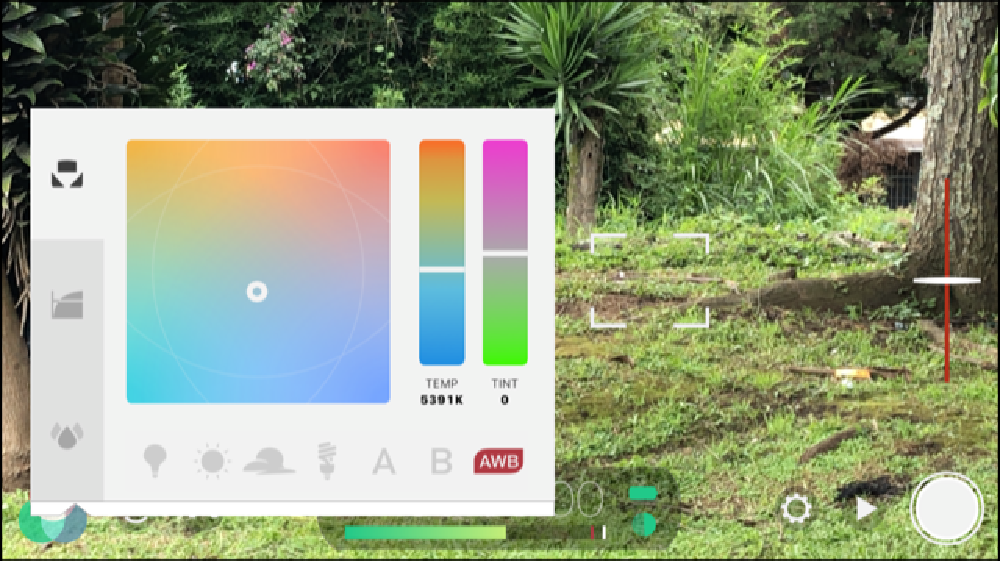
\includegraphics[width=.40\linewidth]{protocol5} \\
  (a) & (b) 
  \end{tabular}
  \end{minipage}
\caption[Whitebalance configuration]{Whitebalance configuration: In a) the automatic white balance is displayed and in b) the fixed white balance.}
\label{fig:whitebalance}
\end{figure}

\subsection{Proper use of the gimbal}

The following are some recommendations for optimal use of the gimbal.

\begin{enumerate}
 \item Make use of a tripod that allows you to make a gimbal grip with both hands.
 \item Tilt the device slightly forward in order to have greater stability during video capture.
 \item Make slow and constant movements. The suggested way of walking with the gimbal is to slightly bend the knees to have greater cushioning of the steps and avoid sudden movements of the camera.
\end{enumerate}

\subsection{Pre-capture application settings}

In order to avoid as much as possible the effect of blurring that can cause the taking of a moving video, it is recommended to set the frame rate of the application to 120 FPS and thus achieve a slow motion effect.



  %----------------------------------------------------------------------------
  \backmatter
  %----------------------------------------------------------------------------

  \printindex                % insert index into document. Don't forget to call
                             % "makeindex filename" first.
\end{document}
